\declarecommand{\dentry}{dentry}
\declarecommand{\dentries}{dentries}
\declarecommand{\Dentry}{Dentry}
\declarecommand{\Dentries}{Dentries}
\declarecommand{\vnode}{{\tt vnode}}
\declarecommand{\vnodes}{{\tt vnodes}}
\declarecommand{\dcache}{{dcache}}
\declarecommand{\inode}{{inode}}
\declarecommand{\dnlc}{{\tt DNLC}}
\declarecommand{\fnone}{{X}}
\declarecommand{\fntwo}{{Y}}
\declarecommand{\fnthree}{{Z}}
\declarecommand{\fnfour}{{A}}
\declarecommand{\fnfive}{{B}}
\declarecommand{\fnsix}{{C}}
\declarecommand{\lnone}{{L}}
\declarecommand{\lntwo}{{R}}
\declarecommand{\completeflag}{{\tt DIR\_COMPLETE}}
\declarecommand{\lookupflag}{{\tt NEED\_LOOKUP}}

\declarecommand{\ubuntuver}{{14.04}}
\declarecommand{\linuxver}{{3.14}}
\declarecommand{\prefixcheckcachesize}{{4}}
\declarecommand{\PCCsize}{{64 KB}}
\declarecommand{\lookuptablesize}{{64}}
\declarecommand{\lookuptableway}{{2}}

\declarecommand{\statspeedup}{{26}}
\declarecommand{\openspeedup}{{13}}
\declarecommand{\slowpathcost}{{xx}}
\declarecommand{\dentryoldsize}{{192}}
\declarecommand{\dentrynewsize}{{192}}
\declarecommand{\dentrysizeoverhead}{{64}}
\declarecommand{\dovecotspeedup}{{12}}
\declarecommand{\gitspeedup}{{7}}
\declarecommand{\updatedbspeedup}{{29}}

\newcolumntype{L}[1]{>{\raggedright\let\newline\\\arraybackslash\hspace{0pt}}m{#1}}
\newcolumntype{C}[1]{>{\centering\let\newline\\\arraybackslash\hspace{0pt}}m{#1}}
\newcolumntype{R}[1]{>{\raggedleft\let\newline\\\arraybackslash\hspace{0pt}}m{#1}}

\chapter{Optimizations in Legacy Operating Systems}
\label{chap:dcache}

This chapter describes the formal definition of the \graphene{} host ABI.

\section{Basic Definitions}

The \graphene{} host ABI defines a set of {\em functions}, similar to the API of UNIX or POSIX.
The functions are directly called by the library OS, along with the arguments given either in the registers or on the stack.
A host-specific \graphene{} loader is responsible for resolving the linking, from the library OS to the host ABI.
\papersection{Challenges for Partitioning with Enclaves}
\label{sec:background}
In this section, we will give a brief overview of \sgx{}, and discuss 
the key challenges developers face when trying to manually partition applications using a technology such as \sgx{}.
%discuss the programming models and threats to security of \sgx{} enclaves.

\papersubsection{Background on \intel{} \sgx{} Enclaves}

\intel{} \sgx{} ({\it Software Guard Extension})
is a set of new x86/x64 instructions
introduced in the \intel{} Skylake processor family.
Using \sgx{}, an 
application can designate part of its virtual memory as an {\em enclave}.
The CPU guarantees that the contents of the enclave never leave the CPU package unencrypted.
The CPU also measures the integrity of a binary loaded into the enclave, and offers remote attestation,
similar to a TPM\fixmedp{cite}.

%%% create a protected memory region, called an {\em enclave}, inside it's virtual memory,
%%% where it can load its security sensitive data with hardware-enforced isolation from the untrusted OS. 
%%% The processor with \sgx{}
%%% guarantees that any data loaded in enclave
%%% stays encrypted in the DRAM, by using a secret key deterministically derived from the application's cryptographic measurement and the CPU secret. 

\sgx{} is an appealing tool for protecting small amounts of highly-sensitive data or code, because it can defend 
against a malicious or compromsed OS, hypervisor, or even hardware peripheral.
For instance, \fixmedp{Foo} et al.~\fixmedp{cite that \sgx{} workshop paper} show how \sgx{} can be used
to build a trusted path from a video chat application to a GPU and network card, which maintains confidentiality and integrity of the
video stream, even if the OS is compromised.
Simlarly, because DRAM contents are encrypted, \sgx{} can resist cold-boot attacks~\cite{halderman09coldboot} or 
malicious peripheral devices~\cite{hudson15thunderstrike}.


%%% \sgx{} also proves the integrity of loaded binaries to remote trusted entities
%%% using mutual attestation based on a symmetric key generated from the measurements of communicating entities.
%%% \sgx{} usage model mostly involve the launched enclave mutually attesting the trusted host
%%% to obtain provisioning of security-sensitive information
%%% through a trusted channel. Such an execution model leverages resources such as CPU and DRAM from vulnerable untrusted \sgx{}-enabled hosts owned by cloud providers
%%% by extending the trust from
%%% the hosts owned and trusted by the clients or service providers.
%%% For instance, \sgx{} can isolate the decoder engine in an enclave
%%% after authenticating the customers to enforce Digital Right Management (DRM) even if the digital data is hosted on an untrusted cloud server.

%Use cases of \sgx{} mostly involve the launched enclave
%retrieving a cryptographically signed attestation from the processor,
%to exchange security critical information with remote servers through secured channels.
%The effect is equivalent to expanding the trusted space from remote servers
%to the local end, to harness local resources such as CPU and DRAM.

%One must note that \sgx{} only promises the integrity of application binaries
%initially loaded in enclaves.
%The gap between integrity of binaries and complete security has to be filled
%by ones who develop and approve the applications.
%More specifically, the clients are responsible of
%testing whether the applications contain any vulnerabilities
%that lead to information leak.
%To minimize the risk of leaving any flaws in the applications unintentionally,
%developers often tend to cut down the trusted computing base (TCB)
%of the applications. With smaller TCB, clients who launched the enclaves
%can more easily reason about the thoroughness of securing the execution.

%%% The key strength of \sgx{} enclaves over other software-based isolation framework such as
%%% {\em Flicker}, {\em Inktag} or {\em Virtual Ghost} is
%%% the ability to defend against attacks at the hardware level.
%%% These software-based solution often
%%% rely on a hypervisor below the OS to isolate the applications.
%%% If the hardware is attacked,
%%% the attackers may still bypass the software checkpoints,
%%% or directly steal confidential information from the DRAM.
%%% For \sgx{}, the only hardware included in the TCB is the CPU package,
%%% and in practice CPUs are believed to be hard to attack.
%%% Using techniques like cold-boot attacks~\cite{halderman09coldboot}
%%% to peek into DRAM content,
%%% or intruding the boot process using corrupted peripheral devices like Thuderstrike~\cite{hudson15thunderstrike}
%%% will affect any software-based isolation, but not \sgx{} enclaves.

\paragraph{Non-Partitioned Applications.}
One approach to using \sgx{} is to run an entire application in the enclave.
This is exemplified by Haven~\cite{baumann14haven}, which runs a \win{} application and all supporting libraries
on top of a {\em library OS}.  This approach is illustrated on the left side of Figure~\ref{fig:libosvssdk}.
The library OS approach does not require any application changes, but bloats the TCB \fixmedp{Rough number of how big Haven is}.
By pulling millions of lines of extraneous code into an enclave, there is a significantly increased risk 
of vulnerabilities that disclose
sensitive data, such as Heartbleed~\fixmedp{cite}.
The library OS approach is useful in its simplicity of deployment and can provide practical benefits, 
such as protecting an application from an untrusted cloud hypervisor.

\begin{figure}[t!]
\centering
\includegraphics[width=\linewidth]{figures/libosvssdk.pdf}
\footnotesize
\vspace{-0.2in}
\caption{
Comparison between the libOS-based model (e.g., Haven)
and the partitioned model for programing applications in enclaves.
Green (light) boxes are trusted components and red (dark) boxes are untrusted.
The libOS-based model yields a larger TCB in the enclave,
while the partitioned model requires developers to be responsible for determining the untrusted interface at the enclave boundary.
}
\label{fig:libosvssdk}
\end{figure}


This paper focuses on a second usage model for enclaves, where the application is partitioned into
untrusted and one or more trusted components (right side of Figure~\ref{fig:libosvssdk}).
Sensitive data and computation are placed inside of enclaves.  This approach requires the developer to
identify sensitive code and data; design and harden an interface between trusted and untrusted components; 
modify the application source; and reason about potential information flows at the enclave boundary.
This effort can be non-trivial and subtle, but for application developers motivated by interests such as 
regulatory compliance or competitive advantage in business, the additional effort can yield a much smaller trusted computing
base (TCB), and thus a reduced attack surface.
A key goal of \sysname{} is to minimize the developer's effort to partition an application---both in lines of 
code changed, and in leveraging language analysis to reason about narrow points in the application's data and control flow.


%To achieve smaller TCB, the software development kit of \sgx{}
%intends to encourage developers to partition the applications and
%keep only security sensitive components in the enclaves.
%Such an intention is exactly contradicted by the trust model of \haven{},
%which must trust the loaded application as a whole.
%Except for the cases in which the whole applications must be secured,
%\haven{} actually downgrades the trustworthiness of enclaves.
%Figure~\ref{fig:libosvssdk} shows the comparison of the two models.

%%% In prior works using \sgx{} enclaves to secure applications,
%%% developers choose between two different programing models: the {\em library-OS-based} and the {\em partitioned} model (as shown in Figure~\ref{fig:libosvssdk}).
%%% In the libOS-based model, developers run the whole standalone,
%%% legacy application inside the enclave, using library OS such as {\em Haven} or {\em Graphene libOS} to facilitate the rich OS features.
%%% The main benefit of using library OS is that developers only have to employ minimal efforts to port any existing application.
%%% Even when designing new applications, developers bear no responsibility
%%% of identifying and reasoning about
%%% the security sensitive part of the application.

%%% However, when using libOS-based model, a sophisticated legacy application
%%% will yield huge trusted computing base (TCB) in the enclave,
%%% aggravating the risk of leaking information through vulnerabilities inside the enclave.
%%% Known bugs such as {\em the heart-bleeding bug} has shown that
%%% running security sensitive code like an encryption engine, and management code such as heart-beating service in the same address space
%%% can cause vulnerabilities that compromise the security by leaking the encryption key.
%%% As a result, using a partitioned model, developers can isolate only the most security sensitive components in an enclave,
%%% and leave the remaining code outside to minimize the TCB.

%%% Developers have to define the {\em untrusted interface} 
%%% to allow parts of a partitioned applications to interact.
%%% The untrusted interface is used either by the the untrusted components
%%% to trigger execution of the isolated components,
%%% or by isolated components to use untrusted rich OS features, such as networking for provisioning and sending the execution output to the remote hosts.
%%% Unlike the libOS approach that has a fixed untrusted interface (for different applications) at their interaction boundary with the OS,
%%% the width of untrusted interface for a partitioned application is up to developers' design.
%%% The \intel{} SDK for \sgx{} supports a set of syntaxes to specify the type and direction of flow for parameters of the untrusted interface, and enforces primitive
%%% type-checking of incoming values on transition to enclave.

%%% The trade-off between the libOS-based and partition model is based 
%%% on ease of development, the width of untrusted interface,
%%% and size of TCB.
%%% The benefit of the libOS-based model is that developers can save the effort
%%% of determining what to execute in the enclave,
%%% and whether the execution is safe,
%%% because the whole application is wrapped in the enclave.
%%% However, the risk of having vulnerabilities in the applications
%%% is not reduced, but in fact amplified due to the addition of
%%% the library OS (e.g., the Haven binary yields around a few hundred MBs) to TCB.
%%% On the other hand, if the developers are willing to spend effort on carefully identifying the untrusted interface and re-designing their application around this interface, the partitioned model can improve security guarantees by minimizing the attack vectors.

%%% The goal of \sysname{} is to provide the benefits of both models.
%%% \sysname{} support a partitioned model
%%% for developers to isolate security-sensitive part of a \java{} application in enclave,
%%% and provide a language-based tool to automatically partition
%%% the minimal supporting classes to generate the enclave image.
%%% Even in the case where the isolated component need to frequently interact with the untrusted component or the OS,
%%% the language protection technique of information flow tracking
%%% guarantees that the secrets in the enclave are never leaked
%%% without the developers explicit consent. 

\paragraph{Side Channels and Denial-of-Service.}
In the current \sgx{} design, side channels are a signficant concern for either the library OS or partitioned model, and are out of the scope of this paper.
A controlled channel attack~\fixmedp{cite} can single step enclave execution by inducing page faults
in the enclave.  \sysname{} does not specifically defend against side channel attacks,
and we expect that any solution to this problem involves redesigning the division of labor in virtual
memory management for enclaves.

Similarly, there is no guarantee that a compromised application will ever enter
an enclave.  Denial-of-service attacks are out of scope for this paper.


\papersubsection{Challenges for Application Partitioning on \sgx{}}

\sgx{} provides useful building blocks for secure applications, but does not
absolve the programmer of any responsibility for reasoning about end-to-end security.
Bugs in the application or supporting libraries can still disclose sensitive data from an enclave,
and porting code into \sgx{} can be subtle.
This subsection outlines several pitfalls in partitioning an application for \sgx{}.

%%% \sgx{} enclaves provide strong isolation guarantee for applications,
%%% against the malicious or vulnerable application components, system stack,
%%% and hardware (except the CPU itself).
%%% However, the security guarantees of the \sgx{} enclave is dependent on whether the developers design perfect applications without exploitable vulnerabilities that may compromise the application's security.
%%% As the application developers are not perfect,
%%% even applications or components isolated in enclave can face threats to their security.
%%% As follows, we discuss a few potential threats
%%% to the enclave security,
%%% even under the assumption that the \sgx{} hardware is implemented as completely secure --- which can be another threat otherwise. 

%\fixmedp{I roughly want the rest of this section to have a problem, explanation, solution structure, with the overall theme being that this is subtle and we really need some analysis tools to get this right}

\paragraph{Writes outside of the enclave.}
\sgx{} allows code inside the enclave to read and write data structures 
outside of the enclave.  Thus, it is easy for a developer to inadvertently write
code that discloses a secret, say by using a library that memoizes intermediate results to the untrusted heap.
A fundamental requirement is that developers must be able to reason about (or assert)
what code can and can't access data {\em outside} of the enclave.
\fixmedp{Can we say anything about whether such tools exist before Civet?}

%\fixmedp{Do I recall correctly that you can easily write to data outside of the enclave?  If so, this seems like something easy to get wrong, especially 
%if a library memoizes intermediate results.  The developer needs to be able to tell 
%Unless I am full of shit, can we paragraph-ize this fixme?

\paragraph{Application vulnerabilities.} 
The major source of threats to enclave security is any internal vulnerabilities in the isolated components,
such as buffer overflows and other memory corruption attacks.
Moreover, although \sgx{} code integrity guarantees make enclaves resistant to code injection,
an attacker may still manipulate control flow using code-reuse attacks~\cite{code-reuse-attacks}.
Moreover, recent research ~\cite{hudata} show that even with perfect control flow integrity,
attackers can still manipulate the execution to leak the secrets through information flow.

Fundamentally, this argues for some combination of static analysis
and runtime monitoring of 
enclave code.  This is greatly simplified when the enclave code is written in higher-level languages
with properties 
%amenable to analysis.
%with type safety, memory safety, and other 
%that provide important 
%safety properties,
such as type safety or memory safety. %, thereby reducing the likelihood of these vulnerabilities.
Ideally, one would formally verify security properties of enclave code~\cite{moat}; this verification is significantly aided by using 
higher-level languages amenable to formal reasoning.
%Verification is significantly harder
%with C or x86 assembly.

%% \paragraph{Applications are not perfect} 
%% The \sgx{} hardware cannot prevent applications from copying secrets out of the enclave without limiting functionality.
%% The trusted isolated components can copy any sensitive data from the enclave to the unencrypted memory, and potentially leak the enclave secrets.
%% The primary risk in the isolated components
%% is often memory corruption vulnerabilities, such as buffer overflow,
%% %Because in enclave applications can access any part of out-of-enclave memory unrestrictedly,
%% prevalent in applications that are not implemented in type-safe languages.

%% The best known technique to prevent vulnerabilities is to model the applications and verify them using {\em formal verification}.
%% While Sinha et.al.,~\cite{moat} use formal verification to prove confidentiality of enclave programs, it is impractical to accurately model complex sophisticated applications.
%% As a result, in addition to formal verification, maintaining smallest TCB
%% in the isolated components is the most practical approach 
%% to ensure enclave security,
%% and is the main reason to choose partitioned programming model over
%% libOS-based model.


\begin{figure}[t!]
\centering
\includegraphics[width=\linewidth]{figures/partition.pdf}
\footnotesize
\vspace{-0.3in}
\caption{
Partitioning --- either manually or by automated tool ---
often causes wider boundary of partition than the actual security sensitivity boundary
due to (a) design granularity : {\tt secHelper} contains a {\tt send()} method that is not partitioned from the rest of the class by design.
The reasons of having the gap vary, for instance, 
that is less security sensitive, but due to the granularity it is not partitioned from the rest of the class or (b) better performance :  the less security sensitive {\tt logger} class is kept in the privileged level to service frequent method calls.
}
\label{fig:partition}
\end{figure}

%However, even if developers partition the applications and run only
%security sensitive components in the enclave,
%the developers may still leave some code irrelevant to
%enclave secrets inside the enclave.
%The reasons of having more-than-minimal TCB in enclaves
%are often that developers have to partition code in the granularity of source files or functions,
%or developers have to import more code to limit the width of interface and
%the frequency of interaction with the untrusted code.

\paragraph{Identifying ``pinch points''.}
Reasoning about where in a program to draw the line between 
trusted and untrusted code is subtle.
On one hand, the developer has an incentive to minimize the size of the 
API between the enclave and untrusted code, as well as an incentive to
minimize the total code in the enclave.  These goals can sometimes be at odds.
Each entry and exit to an enclave has a cost roughly comparable to a
process context switch\fixmedp{right?}; an easy way to reduce enclave entries and exits is to simply 
pull more code into the enclave, which increases the size of the TCB.

\fixmedp{I'm not sure how to explain Figure~\ref{fig:partition}, but it needs an explanation.}

Fundamentally, the art of paritioning an application is to find a ``pinch point'' or
``narrow waist'' in the application, where there is a natural point to insert an API and 
security checks.  This is indeed as much art as science, often done manually by experts\fixmedp{any more supporting evidence or cites?}.
It is unlikely that the average developer will successfully navigate this design process without analysis tools, such as \fixmedp{examples?},
to help identify these natural division points.


%% Experts can use a manual partitioning technique to achieve smallest TCB for the isolated components compared to automated tools.
%% However, the manual partitioning costs a lot of effort,
%% and rare expertise, lack of which can cause larger TCB.

%% Neither manual nor automated partitioning is perfect:
%% the resulted boundary of partitioning often has a gap from the actual boundary of security sensitivity (as shown in figure~\ref{fig:partition}),
%% leaving more code in the privileged level
%% than what's actually needed.
%% Having the gap between the ideal and resulted boundary
%% is mostly inevitable, due to multiple reasons.
%% One common reason is the granularity of partitioning,
%% which can vary from a binary file, a component, a source file,
%% a class, a method (a function) to a line of code.
%% Another reason is that a component or a method may be too frequently called
%% by the security sensitive code,
%% laying the boundary between the component or method from the security sensitive side may bring too much overhead or risk,
%% because the execution crosses the boundary too often.
%% Therefore, developers often will balance among the effort of partitioning,
%% risk or cost of communicating between different partitions,
%% and minimizing the TCB in the security sensitive parts.

\fixmedp{Maybe move the commented paragraph below down into the design section?  I'd like to downplay the plugs for our work here, and instead fulfill these promises later}
%% \sysname{} automates partitioning of applications,
%% based on the boundary at the classes which the developers marked
%% as the interfaces of the enclave.
%% Only the classes that are depended by the marked classes
%% will be included in the enclaves,
%% to minimize the TCB.
%% Although not all classes pulled into the enclaves
%% are necessarily security sensitive,
%% the enclaves are protected from the potential vulnerabilities in those classes,
%% by the security guarantees of \java{} language,
%% and the information flow tracking in \sysname{}.

%Another threat to \sgx{} is the vulnerability of the 
%security sensitive code running in the Enclave. The 
%main guarantee of \sgx{} to isolate the secure data 
%from other components and privileged OS is undermined 
%if the Enclave code can be tricked to leak the 
%security sensitive data to the attacker. Executing 
%buggy code in \sgx{} enclave can inadvertently leak 
%information if the attacker can exploit memory-safety 
%vulnerabilities like buffer overflow and dangling 
%pointers.  

% Cumbersome and approximation to partition code
%The developers have to manually partition their code 
%into security sensitive and insensitive part. If this 
%partitioning is done by a novice developer, some of 
%the security insensitive parts of the application can 
%end up in the security sensitive part, increasing the 
%Trusted Computing Base(TCB). Moreover, the 
%partitioning of code is not straightforward, which 
%can also contribute to a less stricter TCB. The bigger the TCB, the more %vulnerable is the Enclave code to attacks.

% Buggy Code leads to inadvertant information leakage


% \sgx{} code only Integrity protected not confidential
%Moreover, \sgx{} only protects the integrity of the enclave code. The security critical part of the application is stored in plaintext while the secret data is provisioned securely after attestation. However, \sgx{} does not protect the confidentiality of enclave application code which may be executing a secret algorithm. \fixmebj{Talk more about the problem motivating security tag preservation.}
%\sgx{} can natively guarantee either code integrity or
%code confidentiality (as part of the enclave data), but not both.
%If application code is included in the enclave measurement and
%verified by the hardware,
%the code must stay in plaintext as part of the enclave image.
%If any code is stored or provisioned in encrypted forms,
%the application or infrastructure in enclave must dynamically load
%the code after decryption.
%Supporting dynamic loading makes enclaves open to code injection
%if the applications have exploitable vulnerabilities.

\paragraph{Code Integrity {\em and} Confidentiality.} 
The hardware-level \sgx{} code integrity mechanism is based on a cryptographic
signature of a static binary in plaintext.
If any application dynamically loads any code after the enclave's initial measurement,
the initial application must be trusted to attest the loaded code.
The subtle tension is that there is no way to protect the confidentiality of
a secret algorithm, except by dynamically loading an encrypted binary.
Dynamically loading code increases the risk of code injection attacks and other control flow compromises.

Any application partitioning solution that protects sensitive algorithms
must have a robust dynamic loader that can measure encrypted libraries or classes.
\sysname{} includes a loader that can measure encrypted class files,
provisioned from a trusted host.

%% \sgx{} enclaves require code integrity in the isolated applications.
%% If the code integrity is not maintained, adversaries can corrupt the enclave code to
%% force the applications to leak the information provisioned from the remote,
%% trusted hosts.
%% \sgx{} hardware only guarantees
%% the integrity of the code initially loaded into the enclaves.
%% However, if an application choose to dynamically
%% load any code after the enclave starts,
%% the application is responsible for the integrity of the code loaded.
%% The fact that dynamic loading of applications, libraries or components
%% is a feature that can potentially make enclaves vulnerable and open to code injection,
%% raises concerns against supporting managed languages in the enclaves.

%% On the other hand, code confidentiality can be a desirable feature,
%% for application developers who prefer keeping the secret sauce of their algorithms concealed.
%% To enable the feature of code confidentiality in enclaves, the protected code must be dynamically loaded into the enclave,
%% because the \sgx{} hardware only accept
%% the initial loaded code to be in plaintext.
%% \sysname{} provides both code integrity and confidentiality by verifying
%% every classes dynamically loaded into the enclaves,
%% and allows loading classes provisioned from trusted hosts.


%% In general \sgx{} enclaves are prone to having side channels, such as timing channels. Because \sgx{} relies on the untrusted OS for paging,
%% an enclave will always leak page fault addresses, except the lower 12 bits (offsets in pages).
%% Such a leakage gives the untrusted OS to amplify the side channels,
%% by forcing page faults on every instruction or memory access.
%% This so-called {\em Controlled Channel Attack} is common to all applications who use \sgx{} protection, regardless of the programming models.
%% \sysname{} does not specifically defend against side channel attacks.

%% \paragraph{Denial-Of-Service Attacks}
%% \sgx{} is not designed to be safe against denial-of-service attacks.
%% Because the untrusted OS still controls the host resources,
%% there are countless ways to prevent an enclave from making progress.
%% For example, the OS can simply starve the enclaves by
%% never scheduling CPU, memory or other resources to the enclaves.
%% \sysname{} does not specifically defend against denial-of-service attacks.

\paragraph{Discussion.}  This
section has outlined several pitfalls for developers of partitioned applications.
These common pitfalls render the hardware protections of \sgx{} useless.
Language-level analysis can automate error-prone reasoning in the best case, or, in the worst case, 
can at least offer invaluable guidance to the developer.  For \sgx{}-style
hardware to be useful to a wide array of developers, developers need language-level
tools that can also factor in hardware-level protection mechanisms.



%- Motivate the problem.
%- List all attack vectors
%- How can JAVA help?




















































































\section{Minimizing Hit Latency}
\label{sec:dcache}

This section describes
%The first category of optimizations we describe are 
algorithmic improvements to the dcache hit path.  
In the case of a cache hit, one of the most expensive operations
is checking whether 
a process's credentials permit the process to search
the path to a \dentry{} top-down (called a {\bf prefix check}).
This section shows how the hit latency can be significantly reduced
%(by 26\% in our \microbench{}s)
by caching prefix check results.
%this particularly expensive data structure traversal in the common case.
This section explains the optimization, how it is integrated into the existing Linux directory cache 
framework, how these cached results are kept coherent with other file system operations,
and how we use path signatures to further accelerate lookup.


% Should we justify the cost of the search component with measurement?

\subsection{Caching Prefix Checks}
\label{sec:dcache:prefixcheck}

\begin{figure}[t!]
\centering
\includegraphics[width=5.5in]{dcache/figures/dcache-structure.pdf}
\footnotesize
\caption[Optimized Linux directory cache structure.]
{Optimized Linux directory cache structure. \dentries{} are chained in hash buckets. To index the hash bucket for a target \dentry{}, the original lookup routine {\tt d\_lookup} uses a hashing function with key as a combination of the pointer to parent directory and file name ({\em slowpath}).
Our {\em fastpath} hashes the full canonical path of target file to look up the \dentry{}
in the Direct Lookup Hash Table,
and checks the per-credential Prefix Check Cache.}
\label{fig:dcache}
\end{figure}

%\fixmedp{update the picture with new tables}
Like many Unix variants, Linux stores cached path-to-inode mappings (\dentries{}) in a hash
table (\S\ref{sec:dcache:background:dcache}).  This hash table is keyed by a combination of 
the virtual address of the parent \dentry{} and the next path component string, illustrated in
Figure~\ref{fig:dcache}.  
Virtual addresses of kernel objects do not change over time and are identical across processes.
%Each path component is checked for search permission in a top-down fashion,
%which we call a {\bf prefix check}.
%For instance, to look up component {\tt alice} in {\tt /home/alice/foo.txt},
%the kernel would take the virtual address of the \dentry{} for {\tt /home}, 
%and hash it with the string ``alice'' in order to find the bucket to search
%for the \dentry{} mapping ``alice'' to an inode, in order to check search permission on 
%the {\tt alice} directory.
%The latency of a prefix check, and thus a lookup, 
%grows linearly with the number of path components in the prefix.

In practice, prefix checks have a high degree of spatial and temporal locality,
and are highly suitable for caching,
even if this 
means pushing some additional work onto infrequent modifications of the directory structure (e.g., {\tt rename} of a directory).
RCU already makes this trade-off (\S\ref{sec:dcache:background:dcache}).

%Application file access patterns exhibit substantial temporal and spatial locality.
%Moreover, lookups (i.e., reads of the directory hierarchy)
%are vastly more common than modifications of the directory structure (e.g., {\tt rename} of a 
%non-empty directory) or permission changes within the directory structure (e.g., {\tt chmod} or {\tt chown} of a directory).


%% dp: Maybe cut this. Kind of meh
%% Caching prefix checks is analogous to caching access permissions along with 
%% virtual-to-physical translations in a hardware 
%% translation lookaside buffer (TLB). 
%% For instance, each level of an x86 page table encodes access permissions 
%% (e.g., read, write, execute, and user/kernel).  As the hierarchy grows deeper with larger address spaces
%% and hardware virtualization support~\citep{intel10, nestedpagetables}, 
%% needless loads can be elided.

%Linux's use of RCU already makes this trade-off (\S\ref{sec:background:dcache}).

In order to cache prefix check results, we must first decouple 
{\em finding} a \dentry{} from the prefix check.
We added a second, system-wide hash table exclusively for finding a \dentry{}, called the {\bf direct lookup hash table (DLHT)}.
%which only stores recently-accessed \dentries{},
%of \fixmedp{directories?}
The DLHT stores recently-accessed \dentries{}
hashed
by the full, canonicalized path.
A \dentry{} always exists in the primary hash table as usual,
and may exist in the DLHT.
The DLHT is lazily populated, and entries can be removed for coherence
with directory tree modifications (\S\ref{sec:dcache:rename}).

\begin{comment}
\fixmedp{proposed change; measure impact}
\fixmetsai{no done yet, and not sure about the impact. In general, if a file (a leaf) is constantly accessed, there is benefit to add it to DLHT.
Also a dentry found on fastpath means all of its ancestors have passed prefix checks, so if only directories stored, we still have to do one more check.}
%We limit the DLHT to directories because only directories 
%can be in a prefix.  Our lookup algorithm always does a second hashtable
%lookup in the primary hashtable for the final path component.
\end{comment}

Each process caches the result of previous prefix checks
in a {\bf prefix check cache} (PCC), associated with the process's credentials
(discussed further in \S\ref{sec:dcache:cred}), which can be shared among processes
with identical permissions.
The PCC is a hash table that caches dentry virtual addresses 
and a version number (sequence lock), used to detect stale entries (\S\ref{sec:dcache:rename}).
When a prefix check passes, indicating that the credentials are allowed to access the \dentry{}, 
an entry is added to the PCC; entries are replaced according to an LRU policy.
A miss in the PCC can indicate a permission denied
or 
%, which we believe is an uncommon case, or, more commonly,
that the permission check has not executed recently.

%The PCC is a hash table to quickly check if a dentry{} is recently prefix-checked.
%% dp: Meh
\begin{comment}
For simplicity, we implemented a set associative cache, resembling the design of a L1 cache in CPU, but a more sophisticated data structure such as
{\em Cuckoo hashing}~\citep{cuckoo04} can be even more efficient. 
\end{comment}
%lookup and insertion time asymptotically constant.
%The PCC is initially 64 entries, and in our current prototype doubles in size, up to a configurable
%maximum size,
%each time it exceeds a 50\% load factor.  
%If the maximum size and load factor are exceeded
%\fixmedp{implement}  





%% We changed the kernel path hashing strategy to 
%% simply hash the entire canonicalized path, rather than hash 
%% the virtual address of the parent \dentry{} and the next path component.
%% Thus, given any path, the kernel can directly look up the \dentry{} 
%% without walking the entire directory hierarchy.

%% We create a separate hash table, which we call a {\bf direct lookup hash table (DLHT)}.
%% When a \dentry{} is being hashed,
%% it is inserted into both \dcache{} hash table and fast lookup hash table,
%% using their hashing functions respectively.


%% Our {\bf first design} includes placing a {\bf prefix check cache (PCC)} into each \dentry{},
%% %which stores the results of up to \prefixcheckcachesize{} prefix checks,
%% %for \prefixcheckcachesize{} credentials who have most recently look up the \dentry{}.
%% which stores limited amount of prefix checks for credentials who have most recently looked it up.
%% Each cached prefix check is stored using one 64-bit word: 63 bits for a credential identifier
%% and one bit for the prefix check result.
%% However, adding prefix check cache largely increases the size of each \dentry{},
%% thus it will compress the total number of \dentries{} that can be loaded into RAM.
%% The prefix check caches in the most popular \dentries{}
%% will be frequently replaced
%% and have a high cache miss rate,
%% while the other ones can remain underused. 
%\fixmedp{If time, figure out how compact we can reasonably make this}
%The credential identifier, detailed in \S\ref{sec:dcache:selinux},
%represents the process's user id, group membership, capabilities, or any other credentials 
%that could have influenced the prefix check results.
%If any process attributes change that could influence a prefix check, the process must also change
%its credential identifier.


%% To improve space efficiency and cache miss rate of popular \dentries{},
%% our {\bf second design}
%% instead places a {\bf \dentry{} lookup table (DLT)}
%% into the Linux {\tt cred} structure (explained in section~\ref{sec:dcache:cred}).
%% The \dentry{} lookup table is a hash-based set-associative table,
%% and each of its entry contains two 32-bit words:
%% one for storing the lower 9th-40th bit of \dentry{} pointer that has been prefix-checked,
%% and the other for caching the sequence counter of the \dentry{} to determine whether it has been updated.
%% %(0 represents the prefix check has failed).
%% For each credential
%% we initially allocate a DLT with \lookuptablesize{} entries split in \lookuptableway{} ways.
%% The table can be dynamically extended if a credential is looking up more \dentries{},
%% and needs to cache more prefix check results. 

%% dp: worth exploring...
\begin{comment}
Thus, given any path prefix, the kernel
has a {\em fastpath} that directly looks up the prefix 
in the DLHT.  The fastpath case looks up the immediate
parent in the DLHT, checks cached permission for the entire prefix 
(described next), and then looks up the file itself in the primary hashtable.
If the fastpath fails, the code falls back on the original Linux lookup algorithm,
using the primary hashtable exclusively, and traversing components one at a time.
\end{comment}

Thus, given any path, the kernel
has a {\em fastpath} that directly looks up the path
in the DLHT.
If the fastpath hits in the DLHT,
the \dentry{} is then looked up in the process's PCC.
If a PCC entry is found and the version counter matches 
the cached counter, the cached prefix check result is used.
%with the same pointer is found and the sequence counter matches with the the \dentry{}, the results of the cached prefix check are used.
If the fastpath lookup misses in the DLHT or PCC, 
or the version counter in the PCC entry is older than the \dentry{}, 
the code falls back on the original 
Linux lookup algorithm (the {\em slowpath}),
using the primary hashtable exclusively and traversing one component at a time.

%\fixmedp{Chia-che, check this}
In the case of a relative path, such as {\tt foo/bar} under directory {\tt /home/alice},
we effectively concatenate the relative path and the path of the current working directory.
To implement relative paths, Linux already stores 
a pointer to the {\tt dentry} of the current working directory
in each process descriptor ({\tt task\_struct}).
Rather than {\tt memcpy} the strings, we store the intermediate state of the hash function 
in each {\tt dentry} so that hashing can resume from any prefix.

%\fixmedp{Chia-che check this; we should handle these cases; hacks are ok}
%\fixmetsai{revisited}
The current design includes two very infrequent edge cases.
First, a \dentry{} could be freed and reallocated with stale PCC entries.
We detect this case by initializing newly allocated \dentries{} with
%the maximum version number,
a monotonically increasing version number,
allowing PCC entries to detect staleness across reallocation.
Freeing a \dentry{} removes it from the DLHT.
Second, a version number can wrap around after every $2^{32}$ initializations of new dentries or
renames, chmods, or chowns
of non-empty directories; 
our design currently handles wrap-around by invalidating all active PCCs.
%entries less than $2^{31}$
%our design uses a garbage collector to scan all existing PCCs to gradually eliminate stale entries. \fixmetsai{need to implement}

\begin{figure}[t!]
\centering
\includegraphics[width=5.5in]{dcache/figures/dcache-data_structure.pdf}
\footnotesize
\caption[Data structures added in Linux for directory cache optimization]
{Data structures added for fast directory cache lookup. To support {\em fastpath} lookup, we add a 88-byte fast dentry structure to the original \dentry{} and a variable-sized PCC structure into {\tt cred}. 
%% dp: meh
%Both structures are aligned to 64-byte cacheline to make lookup cache-friendly.
}
\label{fig:dcache-data-structure}
\end{figure}

Figure~\ref{fig:dcache-data-structure} illustrates the modifications 
to the Linux \dentry{} structure.  The {\tt fast\_dentry}
stores the signature, flags, a sequence count, a mount point,
lists for managing deep directory entries (\S\ref{sec:readdir:deep}),
and a list ({\tt hash\_chain}) for adding the fast\_dentry to a DLHT bucket.
The PCC is added to the kernel credential structure ({\tt struct cred}), %discussed in \S\ref{sec:dcache:cred}),
and stores a tunable number of tuples of \dentry{} pointers and sequence numbers;
the system is evaluated with a PCC of \PCCsize{}.
Because the highest and lowest bits in each \dentry{} pointer are identical,
the PCC only stores the unique pointer bits (8--39 in x86\_64 Linux) to save space.

%% SOSP Space
%% Although caching prefix checks is straightforward as described thus far,
%% this change 
%% causes ripples through the rest of the code, creating several additional challenges, such as 
%% keeping the cache coherent with modifications.
%% The following subsections address these challenges in the course of 
%% explaining the implementation in more detail.

%\fixmedp{Should we talk about signatures here? I'm tempted to push this to another subsection.}
%\fixmedp{Later: Make sure we explain how we shoot down entries somewhere}

% Order of subsections:
%% Credential IDs and generalization
%% Shootdown
%% Signatures and collisions
%% Special cases



%% \fixmedp{Move down...}
%% Permission caching is a simpler approach to determine file permission
%% than merging access rights of all parent directories.
%% The merging approach is used by related works like DLFS~\citep{lensing13dlfs},
%% which can only resolve permission based on
%% credentials of users and groups.
%% It cannot support more sophisticated access,
%% such as SELinux or AppArmor.
%% On the other hand, The permission caching approach requires no effort of
%% implementing permission merging,
%% thus it is able to support any access control,
%% including SELinux and AppArmor.
%% More details of access control support is discussed in section~\ref{sec:dcache:selinux}.

%% Using permission caching, our lookup method can calculate access right of
%% entering all parent directories to access target file,
%% without any sophisticated merging logic.
%% For every security credential, the access right is calculated by forcing
%% the lookup routine to fall back to the slow path at the first access on any file.
%% Because the slow path shares the exactly same logic as the original component-based lookup in Linux kernel,
%% it can rely on the existing routine of access right checking to determine permissions. 
%% This section will discuss more details about permission caching for fast directory cache lookup.

\subsection{Coherence with Permission and Path Changes}
\label{sec:dcache:rename}

When permissions on a directory or the directory structure are changed, such as with {\tt chmod} or {\tt rename},
any cached prefix checks that include this directory must be invalidated.
Our design  ensures the safety of concurrent lookups and changes by 
invalidating relevant PCC and DLHT entries before a change to the hierarchy,
preventing stale slowpath lookups from being re-cached, and leveraging VFS-level synchronization
to ensure correct slowpath behavior.
  
First, we ensure that a fastpath lookup cannot complete with stale data after a change to the directory structure.
Before a mutation, such as a {\tt rename} or {\tt chmod}, the operation 
must recursively walk all children in the \dcache{} 
and increment the {\tt fast\_dentry} version counter ({\tt seq}). % (steps a1--a4).  
The {\tt fast\_dentry} version counter is used by each process's PCC to detect changes to cached prefix checks on a lookup; % (step b2);
incrementing this version counter invalidates all PCC entries for that \dentry{} without directly modifying
each PCC.  
Changes to the directory structure (e.g., {\tt mount} and {\tt rename}) 
also remove \dentries{} under the old and new path 
from the direct
lookup hash table (DLHT).
PCC and DLHT entries are lazily repopulated on the slowpath.
%These paths can be lazily added back to the DLHT on the slowpath.

Second, we ensure that the results of a  stale slowpath lookup cannot be re-added to the DLHT or PCC by using an atomic, global sequence counter ({\tt invalidation}).
The sequence counter is read before and after a slowpath traversal; results are added to the DLHT and PCC only 
if the counter has not changed, implying no concurrent shootdowns.

Third, we use VFS-level synchronization to ensure that slowpaths synchronize correctly 
with the mutation. 
As an example, {\tt rename}
%%Before the rename begins, our code acquires the 
%%  {\tt invalidation\_lock}, invalidates the relevant children, 
%% acquires the appropriate 
%% VFS-level locks, and then releases the {\tt invalidation\_lock}.
%Rename has stricter requirements to ensure atomicity.
%In the case of {\tt rename}, 
acquires both
a global {\tt rename\_lock} sequence lock, along with per-\dentry{}
locks on the old and new parent directory.
When the {\tt rename\_lock} is held for writing, all lookups on the slowpath 
(i.e., the current Linux code)
must lock each \dentry{}
in a hand-over-hand fashion from the root (or current working directory, for relative paths) 
to the target child.
The locks on target \dentries{} obstruct the hand-over-hand traversal until the rename completes.
The {\tt invalidation} counter prevents caching the results of slowpath lookups that already passed 
this point before the \dentry{} locks were acquired.
%The {\tt rename\_lock} is held until all relevant DLHT entries are evicted,
%and our fastpath traversal is also retried if a concurrent rename is detected by the {\tt rename\_lock}'s sequence count.
%In the current Linux VFS, and our {\em slowpath}, 
Our implementation follows the VFS's existing locking discipline to avoid deadlocks;
it adds version counters that detect inconsistencies and falls back on the slowpath.
Thus, 
relevant PCC and DLHT entries are invalidated before the rename begins, blocking the fastpath;
slowpath traversals will block until the rename is complete
and the per-\dentry{} locks are released;
and a sequence counter ensures that only slowpath traversals that observe the new paths can repopulate the DLHT and PCC.



%% SOSP Space
%% Our \dcache{} design deliberately pushes some additional work onto the uncommon cases of 
%% directory permission changes or changes to the directory structure itself, in order
%% to accelerate frequent lookups.

%% dp: SOSP Space cut
%This is illustrated in Figure~\ref{fig:invalidation}.
%In order to invalidate PCC entries that refer to this directory's children, 
%a permission change operation 
%this choice avoids computing and updating
%prefix checks that will not be used.

%% dp: SOSP Space cut
%% Michael finds this hard to follow
\begin{comment}
\begin{figure}[t!]
\includegraphics[width=1.0\linewidth]{dcache/figures/invalidation.pdf}
\vspace{-15pt}
\footnotesize
\caption{Procedure of updating directory trees for {\tt rename}/{\tt chmod} system calls.
The procedure {\color{red} (a)} invalidates the \dentries{} in all PCCs by incrementing the sequence counters {\color{red} (a2)}. The path will be rehashed. {\color{red} (a2)}.
The procedure then walks all child \dentries{} {\color{red} (a4)} and invalidate them {\color{red} (a4)} (but no rehashing).
A global lock will be held for coherence {\color{red} (a1)}.
If later the old path is looked up on the {\em fastpath} {\color{blue} (b)}, the found \dentry{} {\color{blue} (b1)} has a different sequence counter with the current PCC {\color{blue} (b2)}, thus revalidation is needed.
The forced {\em slowpath} {\color{OliveGreen} (c)} will look up the new path hierachically {\color{OliveGreen} (c1)}, check if the global lock is held {\color{OliveGreen} (c2)}, rehash signature {\color{OliveGreen} (c3)} and finally update the PCC {\color{OliveGreen} (c4)}.  }
\label{fig:invalidation}
%\vspace{-10pt}
\end{figure}
\end{comment}

%% Permissions changes are kept coherent  by 
%% causing fastpath traversals to retry on the slowpath when relevant \dentries{} change.
%% Slowpath traversals will always see a correct
%% view of the directory hierarchy via standard VFS-level synchronization.
%% Once a permission change is applied to a directory, the child version numbers are incremented
%% recursively.  
%% Once these changes are applied, any fastpath lookup will notice the difference in version numbers
%% between the child \dentry{} and the PCC entry, and retry the prefix check.

%% There is a brief window between the permission change of a parent and the version number change to a child.
%% A fastpath traversal during this time is equivalent to executing just before the permission change, which we consider acceptable, as no additional permissions can be acquired
%% and this window is quite short.
%% Similarly, a slowpath lookup  can start before the permission change, 
%% see the old value, and complete just after a permission change.
%% We prevent slowpath lookups from recreating potentially stale PCC entries
%% values by using a global sequence lock ({\tt invalidation\_lock}).



%We also increment the version counter on all children {\em before}
%the rename begins, and hold the
%Once a path is evicted from the DLHT, it 


%% dp: I think this is false
%A positive externality of this design is that the fastpath is never blocked by the {\tt rename\_lock} while {\em slowpath} can be forced to retry.  



\begin{comment}
\fixmedp{moved down from above (too early); dumped para here for now}
When directory structure changes, new prefix check result must be merged
onto every \dentry{} in the directory.
%In order to minimize the penalty on modifications,
We choose to lazily update the prefix check results, by preserving the original
component-based lookup algorithm as a fallback
while we temporarily block directly looking up the \dentries{} until the next access.


In the case of operations that influence a potentially-cached prefix check,
namely {\tt rename}, {\tt chmod}, {\tt chown},
and changes to security-relevant extended attributes,
we must clear the cached prefix check results on all descendants.
The way to clear cached prefix checks (or``to invalidate")
without actually zeroing any structures
is to force aging the sequence counters in the \dentries{}.
Specifically for {\tt rename}, we must also rehash all descendants in direct lookup hash table, because their canonical paths will also change.
\end{comment}

These recursive traversals shift directory permission and structure changes 
from constant time to linear in the size of the sub-tree.
As one example, 
%We found a simple recursive of the subtree to invalidate or rehash all descendants
%can be expensive in a deep directory.
 to {\tt rename} or {\tt chmod} a directory that has
10,000 descendants with at most depth of 4
takes roughly 330 microseconds to complete. 
%\fixmedp{updated numbers}
In the original Linux kernel, {\tt rename} and {\tt chmod} are nearly constant-time operations, and only take 4.5 and 1.1 microseconds.
A few applications, such as {\tt aptitude} or {\tt rsync},
rely on {\tt rename} to atomically replace a directory, 
but this is a small fraction of their total work % done even by these applications,
and orders of magnitude less frequent than lookups, making this a good trade-off overall.

\begin{comment}
The performance penalty for \fixmedp{app example} is \fixmedp{XX\%}.
\S\ref{sec:eval} includes more detailed measurements of these costs and the benefits of constant time lookup, indicating 
that this cost is acceptable.
\end{comment}
%We found a simple recursive walk of the subtree sufficient for our implementation, adding 12--16\% overhead 
%to {\tt chmod} of a directory---a very infrequent operation.
%To serialize readers, we hold the the parent dentry lock on the modified directory,
%which blocks the lookup slowpath until the modification is complete.
%Fast-path lookups which observe the old cached permissions are essentially serialized before the permission change.
%Subsequent executions of the slowpath will repopulate these caches.

\paragraph{Directory References.}
%\fixmedp{Chia-che check}
Unix semantics allow one to {\tt cd} into a directory, and continue
working in that directory after a subsequent permission change 
would otherwise prohibit further accesses.
%hold a reference to a file or directory
%after a permission check that 
%with an opened handle or the current working directory.
For instance, suppose a process is in working directory {\tt /foo/bar}
and {\tt foo}'s permissions change such that the process would not
be able to enter {\tt bar} in the future.
The process should be able continue to open files under {\tt bar}
as long as the process does not leave the directory or exit.
Similar semantics apply to open directory handles.
%Our solution must handle this use case without overriding the premission change.
%\fixmetsai{Don, I rewrote this part to reflect the current design. See if it make sense.}
In our design, such a permission change would ultimately result in a blocked PCC entry,
and a fastpath lookup would violate the expected behavior.
Our design maintains compatibility by
checking if the open reference is still permitted in the PCC.
If the PCC has a more recent entry that would prevent re-opening this handle,
the lookup is forced to take the 
the slowpath, and this stale result is not added to the PCC.

%If a PCC entry for {\tt /foo/bar} is inserted after {\tt /foo}'s permission change, future access to {\tt /foo/bar} will be allowed even after leaving or closing {\tt /foo}.
%This idiosyncrasy of isolating a working directory is supported by 

%If PCC no longer permits the current working directory or base handle, user can still look up paths inside the directory using 
 
%Our current prototype supports this idiosyncrasy by storing the version number
%of the current working directory as of the last {\tt cd};
%if the PCC entry is potentially newer, we only allow the slowpath 
%until the next {\tt cd}, for backward compatibility.
%We believe this is a case where the implementation has leaked into the interface,
%and a reasonable alternative in this situation would be to return an error, such as a stale file handle.

%% \paragraph{Updating Permissions.}
%% Access right of reaching a directory entry is determined by cached permissions
%% calculated in the slow path.
%% When the permission of a directory changes,
%% the kernel must invalidate all prefix check cache in every directory entry under the tree rooted at the directory,
%% to guarantee upcoming access to one of the directory entries be forced to
%% fall back to the slow path for recalculating the permission.

%% Invalidating of prefix check caches is required in two conditions:
%% \begin{compactitem}
%% \item Access permission of a directory is changed by {\tt chmod}, {\tt chown} or other system calls.
%% \item A directory is moved under a different parent directory.
%% \end{compactitem}
%% When invalidation is necessary, the kernel will traverse the whole tree of \dentries{} under the target directory,
%% and mark all \dentries{} as {\tt DENTRY\_INVALIDATED}.
%% If the {\em fastpath} finds a marked \dentry{}, it will fall back to component-based lookup,
%% which flushes the prefix check caches, unmark the \dentry{}, and revalidate the access permission. 

\begin{comment}
In order to mitigate the overhead on {\tt rename}, we push the work of rehashing onto the slowpath.
Because {\tt rename} also clears cached prefix checks,
any following lookup of the descendants
will be forced to fall back to hierarchical slowpath,
which can update direct lookup hash table complimentary.

Because we only invalidate \dentries{} at the operations like {\tt rename} and {\tt chmod}, and force consequential lookup to fall back to slowpath,
consistency of the directory structure is always maintained even if the operations happen concurrently.
The only exception is when a slowpath walk starts before a recursive invalidation happens,
and update a \dentry{} using wrong prefix check after it is invalidated,
the newly cached result will be counted as valid.
To prevent this scenario, we use a
global {\tt invalidate\_lock} sequence lock
to block prefix check caching
whenever an invalidation is in action.
This design is similar to the {\tt rename\_lock} used in the Linux kernel.

%\fixmedp{I see mount/umount as a case of shooting down entries.  I think the text below should be 
%merged in with rename discussion (although there are two sorts of shootdown)}
%\fixmetsai{The two kinds of shootdown is fundamentally different, because invalidation is to force lookup to fall back, but disconnection is to skip dentries while looking up.}

%Because dentries in our prototype are hashed by full path, rather than their parent pointer and file name,
%we must also recursively rehash all children and clear the prefix check cache when a 
%directory is moved.
%We find that this recursive traversal only increases the cost of a {\tt rename} by about 1\%.
% under a different directory.
%\fixmedp{Revisit if we save S4}

Because recursive invalidation can still be an major latency issue on some systems,
we provide an optimization to hide the overhead in the background
and remove penalty on the latency of operations that needs recursive invalidation.
The optimization use a kernel task to handle recursive invalidation
offline with spared CPU cycles.
The only caveat is that fastpath must be {\em disabled} when any invalidation is in process.

Finally, Unix specifies that when a file system is mounted over a non-empty directory,
all files or subdirectories under the directory will be disconnected from the system,
and become unavailable until the file system is unmounted.
We modify {\tt mount} to recursively invalidate all child \dentries{}.
When the file system is unmounted, these \dentries{} can be found again on slowpath and be resurrected for fast lookup.
\end{comment} 


%\paragraph{Disconnecting Directory Entries after Mounting.}
%Unix operating systems allow file system be mounted at any existing directories
%in the system.
%If the directory where mounting happens is not empty,

%In the original design, disconnecting \dentries{} is simple.
%Because all \dentries{} are looked up from their parents,
%disconnecting the root \dentry{} will automatically make all other \dentries{} in the tree unavailable.
%Our solution is to force a tree traversal to mark
%all \dentries{} under the tree as {\tt DENTRY\_DISCONNECTED}.


\subsection{Accelerating Lookups with Signatures}
\label{sec:dcache:collision}
\label{sec:dcache:signatures}

Our optimized lookup uses 240-bit signatures to minimize the cost of
key comparison.
Linux looks up \dentries{} in a hash table with chaining.
When the hash table key is a relatively short path component, the cost of simply 
comparing the keys is acceptable.  However, a full path on Linux can be up to 4,096 characters,
and comparing even modest-length strings can erode the algorithmic benefits of
direct lookup.
We avoid this cost by creating a signature of the path, which 
minimizes the cost of key comparisons.
%can 
%identify a path more compactly and 
%within a bucket of the direct lookup hash table.  

Using signatures introduces a risk of collisions, 
which could cause the system to map a path onto the wrong \dentry{}.
We first explain how signature collisions could cause problems in our design,
followed by the required collision resistance properties,
and, finally, how we selected the signature size to make this
risk vanishingly small.

%We use the multilinear~\citep{lemire2013strongly} 2-universal hash function to generate 192-bit signatures,
%a size selected to make the risk of a signature collision vanishingly small (analysis below).

%% Our fast lookup method uses a hashing function to map canonical paths of files
%% into indexes of hash buckets where the target directory entries are chained.
%% Because the number of hash buckets is limited,
%% collision will almost always happens.
%% In other word, two or more directory entries are often chained in the same hash bucket.
%% To correctly look up the files,
%% a collision detection method is necessary for differentiating directory
%% entries that matches the queried canonical paths.

%% We start with a naive solution of collision detection,
%% by store canonical paths in directory entries
%% and compare them against the queried paths during the lookup.
%% Although path comparison is always accurate
%% on differentiating directory entries,
%% storing canonical paths has expensive cost on memory space, and path comparison can significantly slows down the fast path.
%% The overhead of path storing and comparison may be smaller if the file system
%% has only very short paths,
%% but we cannot make any assumption of average path length in the system. 

%% A better solution of collision detection than path comparison
%% is to use a secondary hashing function to generate signatures of paths.
%% In this solution, each directory entry will have its signatures generated at allocation,
%% and stored inside the entry.
%% To look up a queried path, the lookup routine will map the path (canonicalized)
%% into the target signature
%% and compare it against directory entries in the hash bucket.
%% Because a signature is mostly shorter than the canonical path it represents,
%% storing and comparing it will have a lower overhead
%% on memory space and lookup time.

%%% dp: Although we are right to beat these guys up, I think it is a little too defensive
%%%     Let's save this for the rebuttal if needed
%% Unlike the path comparison solution, the signature-based solution can still cause
%% collision, but at a lower probability.
%% Although the signature-based (or hash-based) solution can be seen in several related work
%% such as DLFS~\citep{lensing13dlfs},
%% many of these works tend to underestimating the probability of collision.
%% Based on our verification, the system described in DLFS
%% actually have higher probability of collision than what the authors claim,
%% and cannot survive in systems that create millions of files. 
%% However, we prove that the signature-based solution can
%% actually be safe to use in our solution of file system directory cache lookup,
%% and the probability of signature collision is truly negligible.

%% dp: Let's start with the risks


\paragraph{Signature collisions.}
When a user looks up a path, our design first calculates a signature
of the canonicalized path, looks up the hash in the global DLHT,
and, if there is a hit in the DLHT, 
looks up the dentry and sequence number in the per-credential PCC.

A user can open the wrong file if the \dentry{} for another file 
with the same signature is already in the DLHT, and that \dentry{} is in the PCC.
For example, if Alice has opened file {\tt /home/alice/foo} with signature X,
and then opens file {\tt /home/alice/bar} that also has signature X,
her second open will actually create a handle to file {\tt foo}.
This creates the concern that a user might corrupt her own files through no fault of her own.  
%For instance, Alice might attempt to open a document for work and overwrite a photo she was just viewing.
This risk can be configured to be vanishingly small based on the signature size (discussed below).



Any incorrect lookup result must be a file that the process (or another process
with the same credentials) has permission to access.
For a fastpath lookup to return anything, a matching \dentry{} pointer must be in the task's PCC,
which is private to tasks with the same credentials.
Thus, a collision will not cause Alice to accidentally open completely irrelevant 
files that belong to Bob, which she could not otherwise access.

%\fixmetsai{Don, I am moving this paragraph here, since it looks like a direct follow-up to the previous paragraph.}
Our design correctly handles the case where 
two users access different files with the same signature,
because misses in the PCC will cause both users to fall back on the slowpath.
%Our design does best-effort collision detection when two users access different files
%with the same signature.
Suppose Bob has opened {\tt foo}, which collides with Alice's {\tt bar}.
When Alice opens {\tt bar}, its signature will 
match in the DLHT, but will miss in the PCC.
This causes Alice's lookup to take the slowpath
to re-execute the prefix check,
ultimately opening the correct file and adding this \dentry{} to her PCC.
%The prefix check will return a result and a pointer to the dentry 
%for {\tt bar}, which is added to Alice's PCC.
%Alice will use this cached \dentry{},
%pointing to the correct file ({\tt bar}), not Bob's {\tt foo}.
Thus, if Bob were adversarial, he cannot cause 
Alice to open the wrong file by changing dcache-internal state.
% experience a collision by influencing dcache state,
%except to lower it by evicting Alice's files from the DLHT.

We choose a random key at boot time for our signature hash function,
mitigating the risk of deterministic errors or offline collision generation,
as one might use to attack an application that opens a file based on user input, such as web server.
Thus, the same path will not generate the same signature 
across reboots or instances of the same kernel.
%Based on the expected success rate of a brute-force attack,
%explained below, one could also periodically drop the cache and rekey the signature function,
%although we expect this would only be needed in a system with years-to-decades of uptime and orders-of-magnitude more powerful hardware than current systems.

%% When signatures replace full path comparisons, the concern is that the 
%% kernel may open a different file than the one the user intended.
%% The worst case is when a user, Alice, looks up two different paths with colliding signatures,
%% both take the fast path, and the second lookup returns the first file.
%% In this case, Alice cannot open any files she couldn't otherwise access, but may open the wrong file.
%% %In the rare event this happens, all permission checks will execute correctly, 
%% %so the user cannot access any files she couldn't otherwise access.
%% Signature collisions are detected on the {\em slowpath},
%% which is always taken the first time a user accesses a given path; colliding paths are permanently blocked from the DLHT with a \dentry{} flag.
%% %\fixmedp{add collision detection?}
%% Thus, an adversarial user, Mallory, cannot influence 
%% the risk Alice will experience a collision,
%% except to lower it by evicting Alice's files from the DLHT.
%Finally,
%We mitigate the risk of 
%deterministic errors or offline collision generation 
%by %salting
%using a random key for our signature hash function chosen at boot time, keeping signatures
%hidden from users, and using a collision-resistant hash function (discussed in more detail below).

%% Thus, the one remaining and important concern about optimizing lookup with a signature comparison
%% is that a user might corrupt her own files through no fault of her own.  
%% For instance, Bob might attempt to open a document for work and overwrite a photo he was just viewing.
%% This risk is configurable based on the signature size.  

Despite all of these measures, 
this risk may still be unacceptable for applications running as root,
which can open any file,
especially those that accept input from an untrusted user.
For example, suppose a malicious user has identified
a path with the same signature as the password database.
This user  might pass this path to a setuid-root utility
and trick the setuid utility into overwriting 
the password database.
This risk could be eliminated by disallowing signature-based 
lookup acceleration for privileged binaries or security-sensitive path names,
although this is not implemented in our prototype.

% (generally \fixmedp{XX-YY (bill says 160--256, but no handy cites)} bits)\fixmedp{cites}.

%% Because this is unacceptable behavior, we select a signature such that
%% collisions will be indistinguishable from disk sector corruptions.
%% Although we do not do this in our prototype, 
%% even this risk could be eliminated for 
%% for root processes by using more expensive checks.

\paragraph{Collision Resistance Requirements.}
The security of our design hinges on an adversary only being able to find collisions
through brute force.  
Our design can use either a 2-universal hash function or a pseudorandom function family (PRF)
to generate path signatures.
%; the 
%principal concerns are performance and risk of side channels.
In terms of collision resistance, the difference between a 2-universal hash
and a PRF is that the adversary can potentially learn the secret key 
by observing the outputs of the 2-universal function, but cannot learn the key from 
the outputs of a PRF.
Because our dcache design does not reveal the signatures to the user,
only whether two paths have a signature collision,
a hash function from either family is sufficient.

One caveat is that, with a 2-universal hash function, 
one must be careful that timing and other side channels do not leak 
the signature.  For example, one cannot use bits from the signature
to also index the hash table, as one might learn bits of the signature from 
measuring time to walk the chain on a given hash bucket.
In the case of our selected function, one can safely use the lower bits from 
the 256-bit hash output, as lower bits are not influenced by the values in higher bits in our particular algorithm;
we thus use a 16 bit hash table index and a 240-bit signature.
In contrast, when the signature is generated with a PRF,
concerns about learning the signature from side channels are obviated.

Our design uses the 2-universal multilinear hash function~\citep{lemire2013strongly}.
%and we carefully audit any code that calculates or compares signatures for potential side channels.
We did several experiments using PRFs based on the AES-NI hardware, and could not
find a function that was fast enough to improve over baseline Linux.
% until  paths had 4 or more components. \fixmedp{Still true?}
Using current 128-bit AES hardware, we could improve performance at 4 or more path components,
but creating a 256-bit PRF required a more elaborate construction that is too expensive.
%This was largely because we could not get enough bits from the 128-bit AES hardware without adding more elaborate constructions.
A more cautious implementation might favor a PRF to avoid any risk of overlooked side channels, especially
if a fast, 256-bit PRF becomes available in future generations of hardware.


%% SOSP Space
\begin{comment}
\begin{figure}[t!]
\centering
\includegraphics[width=.7\linewidth]{dcache/plots/hash.pdf}
\vspace{-10pt}
\footnotesize
\caption{
Cycles to hash messages of varying sizes using the 2-universal multilinear hash (mhash) and using the PRF cbc-mac(aes) using the Intel AES-NI instructions.
Lower is better; at lower values, cbc-mac(aes) is roughly twice as slow as mhash. }
\label{fig:hash}
\vspace{-10pt}
\end{figure}

Thus, the main reason to select a 2-universal function over a 
PRF is performance.  
Our design can use a hash function from either family.
Figure~\ref{fig:hash} compares the performance of hashing different message lengths
using the 2-universal multilinear hash function~\citep{lemire2013strongly}  (mhash)
and, as a PRF,
the CBC-MAC algorithm with hardware-accelerated AES
as the block cipher.
Because AES only creates a 128-bit hash value, we ran the algorithm twice with different keys to create a 256-bit output;
as a result, using CBC-MAC(aes) takes roughly twice as long as mhash.
In terms of the impact this has on lookup performance, 
mhash can outperform baseline Linux even for a single-component path,
whereas CBC-MAC(aes) is only faster than Linux with four path components.
We expect that, with hardware support for a 256-bit hash output, a PRF would be equally practical
for our purposes.

In order to realize the best performance, we use the mhash function in our experiments,
and carefully audit any code that calculates or compares signatures for potential side channels.
\fixmedp{Clear this fixme when done}
A more cautious implementation might favor a PRF to avoid any risk of overlooked side channels.
\end{comment}

%% \fixmedp{Educated speculation from here forward.  Revisit once we have numbers}
%% For a PRF, we used the CBC-MAC algorithm to create a signature, using AES
%% as the block cipher.  
%% Because AES only creates a 128-bit hash value, we ran the algorithm twice with different keys to create a 256-bit output.
%% In our experiments, hardware-accelerated AES instructions make the cbc-mac(aes)
%% fast enough to accelerate lookup by \fixmedp{XX\%} for the test in Figure~\ref{fig:by-version}.
%% The 
%% also improves lookup by \fixmedp{XX\%} in this test.
%% Because the improvements from a 2-universal hash are marginal,
%% we err on the side of caution and report only results with a PRF-based signature.


\paragraph{Probability of a signature collision.}
We selected a 240-bit signature, 
which is comparable to signature sizes used in data 
deduplication systems, ranging from 128--256 bits.  Deduplication designs commonly 
select a signature size that introduces a
risk of collisions substantially less than the risk of undetected ECC RAM 
errors~\citep{Debnath:2010:CSU:1855840.1855856, Srinivasan:2012:ILI:2208461.2208485, Quinlan:2002:VNA:645371.651321, Zhu:2008:ADB:1364813.1364831}.

We assume an adversary that is searching for collisions by brute force.
This adversary must lookup paths on the system,
such as by opening local files or querying paths on a web server.
Because our hash function is keyed with a random value and the output is 
hidden from the user,
the adversary cannot search for collisions except on the target system.
Thus, the adversary is limited by the rate of lookups on the system,
as well as the capacity of the target system to hold multiple signatures
in cache for comparison.

%Assuming an adversary is using brute force to find a collision,
We calculate the expected time 
at which the risk of a collision becomes non-negligible (i.e., higher than $2^{-128}$) 
%to find a collision 
%with a 240-bit hash value, and
%Suppose the adversary makes $t$ attempts to look up any paths in the directory cache, 
and model the risk of collision as follows.
First, $|H(X)|=2^{240}$ is
the number of possible signatures.
We  limit the cache to $n=2^{35}$ entries (i.e., assuming 10TB of dcache space in RAM and 320 bytes per entry),
with an LRU replacement policy.
We calculate the number of queries ($q$) after which the risk of a collision is 
higher than $P=2^{-128}$ as follows:
\begin{align*}
q \simeq ln(1 - p) * \frac{|H(x)|}{-n} \simeq ln(1-2^{-128}) * \frac{2^{240}}{-2^{35}} \simeq 2^{77}
\end{align*}
At a very generous 
lookup rate of 100 billion per second (current cores can
do roughly 3 million per second),
the expected time 
%in the brute force attack
at which the probability of a brute-force collision goes above $2^{-128}$
is 48 thousand years.

%% If one does a similar calculation with a completely unbounded 
%% dcache (i.e, each new signature is compared against all previous signatures),
%% the expected time drops to 8 years.
%% In such a worst case, the cache can be dropped and a new random signature key selected
%% after every 8 years of uptime, but with any reasonable bound on the cache size,
%% this should not be a concern.

%% and an uptime of 10 years, for $t \simeq 3.16 * 10^{19}$.
%% We assume an unbounded directory cache.
%% The probability of successfully causing any collision is:

%% \vspace{-0.15in}
%% \begin{align*}
%% P_{Adv}(t,H(X)) \simeq 1 - \epsilon^{-\frac{t^2}{2|H(X)|}}
%% \end{align*}
%% \vspace{-0.15in}

%% Thus, with 192 signature bits, the probability of a collision
%% is less than XXX, which is algorithmically negligible.

%% In order to less than a one in a billion \fixmedp{machines?}
%% the number of attempts by the adversary must be at least:

%% \vspace{-0.15in}
%% \begin{align*}
%% T_{Adv}({10}^{-9},2^{192}) \simeq \sqrtsign{\ln{(1-{10}^{-9})} \times -2 \times 2^{192}} \simeq 2^{81}
%% \end{align*}
%% \vspace{-0.15in}


%% In a system with 10-year uptime, assuming the directory cache is never shrinked, an adversary must perform at least ${10}^{17}$ lookups per second, to achieve one success in a billion manipulated systems. Such an adversary is computationally impossible to succeed in the real world.

%% \fixmedp{I'm confused.  We seem pretty far from $2^{-128}$.  Also, I'm not sure why we are talking about the number of systems.  Let's assume the number of systems is independent and focus on one system, since each has a different random key.}

\begin{comment}

\fixmedp{Chia-Che, please update these calculations.  What happens if we do things Michael's way?}
\fixmedp{once this is resolved, respond to D6}
\fixmedp{Add a note that this is an upper bound and why (just check that what is going on is clear after revision}

We consider two possible collision cases separately.
First, consider the case where two \dentries{} in the cache have a 
matching signature.
This type of collision could cause an application to access the wrong file,
and eventually retrieve wrong content or corrupt the file.
The probability of this type of collision is:
%
\begin{align*}
P_+(n,H(X)) = \frac{n(n-1)}{2} \times \frac{1}{|H(X)|} \simeq \frac{n^2}{2|H(X)|}
\end{align*}
%
where $n$ is the number of directory entries in the system, and $|H(X)|$ is
the number of possible signatures.  

The second type of collision happens if a user 
asks for a path that does not exist in the cache, which 
collides with an existing directory entry
with a different path.
This type of collision will cause the application to
assume existence of a nonexistent file and potentially corrupt other files.
The probability of this type of collision among $q$ queried paths is:

\vspace{-0.15in}
\begin{align*}
P_-(n,H(X),q) = 1 - (1 - \frac{n}{|H(X)|})^q \simeq 1 - \epsilon^{-q\frac{n}{|H(X)|}}
\end{align*}
\vspace{-0.15in}

We argue that the probability of both types of collision is negligible
when using a 192-bit universal hashing function to generate path signatures.
In our assumption, most systems will devote no more than 16GB of physical memory in directory cache, indicating that at most $\simeq 10^8$
\dentries{} will coexist at the same time.
A very busy system with a 10-year uptime, performing an average of 1000 lookup per second,
will query the directory cache for $3\times{10}^{11}$ times ($=q$).
%The number of directory entries is much smaller than
%the number of actual files and directories on storage because directory cache only keeps entries
%that are most recently accessed.
%has the longest possible history of queries.
Using a 192-bit signature, number of possible signatures is ${2}^{192}$ (=$|H(X)|$).
The probability of either collision can be calculated as follows:

\vspace{-0.15in}
\begin{align*}
P_+(10^8,{2}^{192}) \simeq \frac{{(10^8)}^2}{2\times{2}^{192}} \simeq {2}^{-139}
\end{align*}
\vspace{-0.28in}
\begin{align*}
P_-(10^8,{2}^{192},3\times{10}^{11}) \simeq 1 - \epsilon^{-3\times{10}^{11}\frac{10^8}{{2}^{192}}} \simeq {2}^{-128}
\end{align*}
\vspace{-0.15in}

In conclusion, with a directory cache no larger than 16GB, 192-bit signatures make the risk of collision 
negligible within $3\times{10}^{11}$ lookup operations,
or roughly every 10 years.
If a system decides to dedicate more physical memory than 16GB in directory cache,
longer signatures will have to be used,
or a shorter life span of the system must be assumed.
We can enforce this assumption and mitigate the risk of brute force attacks 
by changing the signature key,
and dropping or recalculating the signature for all dcache entries
after this threshold of lookups has been met.

\paragraph{Adversary Resistance.}



Because permission check only happens on the {\em slowpath}, signature collision will never cause security breach with benign users. However, many priviledged processes (e.g. Setuid-to-root programs, system services) in the system can be manipulated by a malicious user to exploit signature collision.
Fortunately, the strength of such an adversary is limited by the system latency, because it cannot perform an offline attack to the signature algorithm, but brute-forcely attempt for lookup in the system.

Assume a stronger adversary uses {\em Birthday Attack} to discover any pairs of paths that have signature collision. Suppose the adversary makes $t$ attempts to look up any paths in the directory cache, the probability of successfully causing any collision is:

\vspace{-0.15in}
\begin{align*}
P_{Adv}(t,H(X)) \simeq 1 - \epsilon^{-\frac{t^2}{2|H(X)|}}
\end{align*}
\vspace{-0.15in}

In other word, to achieve $10^{-9}$ success rate (one in a billion machines), the number of attempts by the adversary must be at least:

\vspace{-0.15in}
\begin{align*}
T_{Adv}({10}^{-9},2^{192}) \simeq \sqrtsign{\ln{(1-{10}^{-9})} \times -2 \times 2^{192}} \simeq 2^{81}
\end{align*}
\vspace{-0.15in}

In a system with 10-year uptime, assuming the directory cache is never shrinked, an adversary must perform at least ${10}^{17}$ lookups per second, to achieve one success in a billion manipulated systems. Such an adversary is computationally impossible to succeed in the real world.
\end{comment}



%The probability of either type of collision is lower than $2^{-128}$,
%which is algorithmically negligible.
%Because mean-time-to-failure (MTTF) of most hard drives ranges from $10^6$ to $1.5\times10^6$ hours~\citep{schroeder07mttf},
%any directory collisions will be indistinguishable from a disk sector 
%failure that corrupts directory metadata.
%\fixmedp{Let's consider dropping the first case for space here.}

%it is guaranteed that any systems will have to restart to recover from disk \fixmedp{sector?} failures before collision happens in the directory cache.

%At high probability, the collision will never appear in the history of queries
%before the system is restarted.

%% The only possible attack using signature collision is to maintain
%% an oracle of all queried paths for brute-force attack across system restart.
%% To defend this attack, we use a randomly generated seed to randomize
%% the hashing function every time the system starts. 

%% In our threat model, we are not defending any offline birthday attack
%% that deliberately queries two paths or creates two files that are known to
%% have colliding signatures.
%% These attacks is not a threat for us because they cannot bypass
%% permission check while accessing the files.
%% In most cases, an adversary that uses birthday attack can only corrupt
%% a file that it already owns the access right.
%% The worst scenarios is that the adversary may trick a seteuid-to-root
%% program to enter a directory which it does not have privilege to.  



\begin{comment}
A good design of caching systems requires a fully optimized lookup method,
which uses the fastest way possible to
determine whether requested data exists in the cache.
Efficiency of the lookup method is especially essential and dominating the
overall lookup performance when
the caching system has a significantly high hit rate.
In the directory cache, a high hit rate can be expected in file systems with temporal locality in file access pattern, low memory pressure
and infrequent metadata relocation.
We predict that these characteristics can be found in majority of systems,
because applications are inclined to access files repeatedly,
and enough spared memory is often available.
These systems will certainly benefit from any improvement on the efficiency of
directory cache lookup.

The directory cache in current Linux kernel uses component-based lookup.
To search for a requested file, the lookup routine will scan and delimit 
every component in path of the file,
and iterate through chained entries in correspondent hash buckets as many times
as the number of components.
The latency of directory cache lookup will grow linearly as longer and deeper
paths are queried.
Despite many efforts have been made in Linux kernel, directory cache lookup
is still one expensive cost to pay in many file system operations. 

We present the design of a significantly faster directory cache lookup
for Linux \linuxver{} kernel.
The lookup method can maximize the speed of searching
a directory entry for a target file which is previously accessed and 
has its metadata cached in memory.


The basic design of our lookup method is simple:
To search the directory entry for a requested file,
instead of breaking the path of file into components and iterates hash buckets repeatedly,
we use a hashing function that maps the whole canonical path of the file
into the index of hash bucket,
and directly look up the directory entry that stores the metadata of the last component.
If the directory entry is found, it is returned immediately to caller routine
for file system operations.
If the directory entry is not found, it is a case of cache miss.
When a cache miss happens, VFS asks file system drivers to locate
and retrieve metadata from the storage.
\end{comment}

%% To deal with cache misses,
%% our solution keeps the original component-based lookup method of Linux kernel,
%% as a slow path to fall back when our lookup method fails searching the
%% directory entry.
%% When a cache miss happen, even if the directory entry for the requested file
%% does not exists in the cache, the parent directories of the file may have been
%% accessed and have their directory entries created.
%% Using component-based lookup as slow path can recollect all created parent
%% directory entries, and request file system drivers to retrieve metadata of the rest
%% of parent directories and the files to cache.
%% Because the file system driver interface of Linux kernel is designed to look
%% up metadata by the parent directory and a file name,
%% using component-based lookup can keep file system drivers unchanged,
%% which can largely alleviate the pain of porting third-party file system driver
%% codes to the new directory cache design.

%% Another reason of using component-based lookup as slow path is to
%% calculate user access right against the target file.
%% To allow an user to access a file, the user requires not only the privileges
%% of file operations,
%% but also permission to enter every parent directory of the file.
%% The easiest way of calculating the permission is to resolve the access right
%% at each parent directory,
%% while looking up entries by each component of the path.
%% Once the permission of a directory or a file is calculated in the slow path,
%% we cache the permission in directory entry
%% and reuse it to determine the access right at next time when
%% the directory entry is looked up in the fast path.
 
%% The permission cached in directory entries is bound to the user credential
%% of process who performs the slow path.
%% If a different user credential look up a directory entry by the fast path,
%% it cannot be guaranteed to have permission to access the file.
%% For example, user {\tt A} and {\tt B} accesses the file {\tt /home/foo/bar},
%% but only user {\tt A} has the permission to entry the directory {\tt /home/foo}.
%% If user {\tt A} has accessed the file first, the kernel will create the directory
%% entry of {\tt /home/foo/bar}, which can be directly looked up in the fast path
%% by user {\tt B}.
%% In these cases of {\bf permission cache miss}, we must
%% force directory cache lookup to fall back to the slow path, in order to calculate
%% the access right for the new user credential.




%% The design of constructing a faster lookup method upon a slower one
%% is comparable to the concept of {\bf TLB (translation lookaside buffer)}.
%% TLB is a hardware optimization of multiple-level page tables traversal
%% in MMU to
%% translate virtual memory addresses into physical pages.
%% By falling back to page table traversal, TLB can recover from incoherence
%% without a sophisticated synchronization and update scheme.
%% The operating system only needs to flush the TLB timely whenever incoherence
%% is suspected or the page table needs to be updated.
%% Similarly, our fast lookup method for file system directory cache works without
%% any logic to update or to sync up directory entries, but simply fall backs to
%% slower component-based lookup to reassure coherence.

%% \paragraph{Expected Speed-up of Lookup Time}
%% Based on expected hit rate, we can predict the average lookup time
%% in directory cache
%% before and after applying the fast path:

%% \vspace{-0.22in}
%% \begin{flalign*}
%% & {Lookup\;time}_{original} = {Time}_{slow\;path} + {Time}_{storage\;lookup} \\
%% & \times (1 - (Hit\;rate))\\
%% & {Lookup\;time}_{optimized} = {Time}_{fast\;path} \times (Hit\;rate) \\
%% & + ({Time}_{slow\;path} + {Time}_{storage\;lookup}) \times (1 - (Hit\;rate))
%% \end{flalign*}
%% \vspace{-0.22in}

%% From the expected lookup times, we can calculate the improvement of performance as follows:

%% \vspace{-0.22in}
%% \begin{flalign*}
%% & {Speed\;up} = \frac{({Time}_{slow\;path} - {Time}_{fast\;path}) \times (Hit\;rate)}{{Lookup\;time}_{original}}
%% \end{flalign*}
%% \vspace{-0.22in}

\section{Generalizing the Fast Path for Lookup}
\label{sec:generalize}

Thus far, we have explained our fast path optimization using the relatively straightforward
case of canonical path names.  
This section explains how these optimizations integrate with Linux's
advanced security modules,
%, such as SELinux~\citep{selinux} and AppArmor~\citep{apparmor},
as well as how we 
address a number of edge cases in Unix path semantics,
%which must be implemented correctly, 
such as mount options, mount aliases, and symbolic links.  
%Linux also includes a number of  which must work correctly with any VFS-level optimizations.
%This section explains how we address these challenges.

\subsection{Generalizing Credentials}
\label{sec:dcache:cred}
\label{sec:dcache:selinux}

%Two key requirements of our dcache optimizations are that they must be general
%and that space overheads for extra metadata must be minimized.
Linux includes an extensible security
module framework (LSMs~\citep{wright+lsm}), upon which SELinux~\citep{selinux}, AppArmor~\citep{apparmor}, and others are built.
An LSM can override the implementation of search permission checks,
checking customized attributes of the directory hierarchy or
process.
Thus, our dcache optimizations must still work correctly even when an LSM overrides the default access control rules.
%the default definition of 
%we need a general mechanism to encapsulate all possible credentials of a process with minimal 
%space overhead in the \dentries{}.

Our approach leverages the {\tt cred} structure in Linux, which is designed to store 
the credentials of a 
process ({\tt task\_struct}), and has several useful properties.
First, a {\tt cred} struct is comprehensive, including all variables that influence default permissions,
and including an opaque {\tt security} pointer for an LSM to store metadata.
Second, a {\tt cred} is copy-on-write (COW), so when a process changes its credentials, such as 
by executing a {\tt setuid} binary or changing roles in SELinux, 
the {\tt cred} is copied.  We manually checked 
that AppArmor and SELinux respect the COW conventions for changes to private metadata.
Moreover, a {\tt cred} can be shared by processes in common cases, such as a shell script forking children with the same credentials.
Thus, the {\tt cred} structure meets most of our needs, with a few changes, which we explain below.

%\fixmedp{Clarify per-process is shared with common cred}

%As explained in Section~\ref{sec:dcache:prefixcheck}, 
We store cached prefix checks (\S\ref{sec:dcache:prefixcheck}) in each  {\tt cred} structure,
coupling prefix check results with immutable credentials.
New {\tt cred} structures are initialized with an empty PCC.
When more processes share the PCC, they can further reduce the number of slowpath lookups.


%% describe two designs of prefix check caching:
%% one is using a prefix check cache in each \dentry{},
%% and one is using a \dentry{} lookup table in each {\tt cred} structure.
%% The former uses a 63-bit integer, called the credential identifier (CID), as a layer of indirection to {\tt cred},
%% while the latter simply places a pointer in {\tt cred} to reference the DLT.
%% Using CID, we must handle the very infrequent case of CID wrap-around.
%% Using DLT, we can avoid handling CID wrap-around, and have better space efficiency as explained in section~\ref{sec:dcache:prefixcheck}.

%to minimize the complexity of freeing and reallocating the {\tt cred} structure itself.
%A simple alternative would have been to simply store the kernel virtual address of the {\tt cred} in 
%various \dentry{} prefix caches, but these caches would have to be cleared before the {\tt cred} is 
%freed, lest a recycled {\tt cred} obtain access to a stale prefix.
%Rather than incur this bookkeeping cost, we simply assign a unique CID integer value to 
%Each time a {\tt cred} is allocated and reused, a new CID is assigned to the cred.
%The CID approach allows stale CID's to safely persist in a prefix cache until they are evicted by LRU,
%and does not complicate freeing a {\tt cred}.

%Using CID, we must handle the very infrequent case of CID wrap-around
%by simply resetting 
%the CID of all active {\tt cred} and clearing all prefix caches.
%We note that, even if an extremely efficient machine changed credentials one trillion 
%times per second
%(cf.\ current cores process at most 4 billion instructions/second),
%a wrap-around would occur once every 106 days. 
%We believe this is acceptable:
%most end-user machines reboot for kernel patches more frequently than this, 
%and even highly-available systems can afford to clear the prefix check cache 
%(not the entire dcache) a few times a year in exchange for the demonstrated benefits.



% reuse
%% The key challenge of implementing permission caching is
%% to identify security credentials within cached permission records in each directory entry.
%% If the access rights of a process are changed, such as updating user/group ID by calling system call {\tt setuid} and {\tt setgid}, or applying new SELinux labels or AppArmor rules,
%% the previous cached permissions should not be
%% reused in the lookup routine if it can cause privilege escalation.

%% Our solution uses the {\tt cred} structure defined in Linux kernel to identify different security credentials.
%% The {\tt cred} structure is a kernel structure referenced by {\tt task\_struct},
%% to store all real/effective user/group IDs, capability, security labels and security records of processes.
%% The {\tt cred} structure can be shared by related threads and processes,
%% so child processes or other threads will not need be forced to recalculate permissions
%% if the directory entry is looked up once by the parent process.
%% Another reason of identifying by {\tt cred} structures
%% is that the {\tt cred} structure in each {\tt task\_struct} is always
%% recreated if the access rights are changed.

%% In order to identify cached permission by {\tt cred} structures,
%% our solution assigns a credential ID to every {\tt cred} structure allocated in the kernel.
%% The credential IDs are allocated incrementally, so they will not be reused soon
%% when {\tt cred} structures are destroyed.
%% Whenever the permission is recalculated, the credential ID of the {\tt cred} structure referenced by the current {\tt task\_struct},
%% will be assigned to the permission cache in the directory entry.
%% The credential ID in permission cache is later used to determine whether the permission can be reused by calling processes.

%Either placing CID or DLT in the {\tt cred} structure,
%it is always beneficial to share cached prefix check with more processes that share the same critical credentials.

One challenge is that Linux often 
allocates new {\tt cred} structures {\em even when credentials do not change}.
The underlying issue is that COW behavior is not implemented in the page tables, 
but rather by convention in code that {\em might} modify the {\tt cred}.
In many cases, such as in {\tt exec}, it is simpler to just allocate another {\tt cred} in advance,
rather than determine whether the credentials will be changed.
This liberal allocation of new {\tt cred}s 
creates a problem for reusing prefix cache entries across child processes 
with the same credentials.
To mitigate this problem, we wait until a new {\tt cred}
is applied to a process ({\tt commit\_creds()}).
If the contents of the {\tt cred} did not change, the old {\tt cred} and PCC is reused and shared.

%Only when Linux Security Module (LSM) specify that the new process has a different credentials,
%CID or DLT will be allocated when
%we defer allocation of the 
%CID or DLT
%the {\tt cred} is actually applied to the process ({\tt commit\_creds()}),
%and only allocate a new CID if the contents have changed.

%\fixmedp{Maybe cut if not implemented?}
%% In order to safely reuse {\tt cred} structures with LSMs,
%% we added a return parameter to the LSM credential initialization hook 
%% to communicate whether the credential changed with respect to prefix checking.
%% This optimization is our only modification to the LSM API and is optional;
%% without this change, we can disable {\tt cred} structure reuse with a LSM.

%%%  is a helpful optimization; without this LSM ch
%%% \fixmedp{How does the LSM determine if cred are equal?  Some function?  I just cut for now}
%%% \fixmetsai{Answered below}
%%% We rely on LSM to specify whether a credential change is relevant to file system traversal.
%%% For example, upon updating application profiles using {\em AppArmor},
%%% or altering {\tt search} permission on directory objects using {\em SELinux},
%%% or simply setting user IDs
%%% or adding {\tt CAP\_DAC\_OVERRIDE} capability to a process,
%%% the LSMs or VFS can mark the PCC in the new {\tt cred} as stale, and force allocating a new PCC at {\tt commit\_creds()}.

%dp: Not impl, not that interesting
%% To further improve reuse of cached prefix check,
%% we track the most recently used {\tt cred} structures in a hash table, keyed by the content of the structure.
%% %% dp: Ok
%% %\fixmetsai{I believe it should be "most recently used cred" because we are exploiting the temporal locality}
%% If a newly allocated {\tt cred} structure matches a recently used {\tt cred},
%% the old {\tt cred} and PCC are reused.
%% %has a matching credential, %according to the LSM,
%% %we can then reuse the CID or DLT.
%% %we then check the hash table for 
%% %a reusable CID.
%% This captures the case where identical credentials appear independently, such
%% as one user with two ssh connections to the system.
%Our solution maintains a credential cache with limited size,
%which can track credential IDs of most recently referenced {\tt cred} structures.
%For each {\tt cred} structure, a signature is generated based on
%all access rights related and can be used to match with the credential cache.
%\end{comment}

%% We predict that permission caching with credential identification is effective
%% on limiting the penalty of lookup performance
%% for recalculating permissions.
%% We observe that temporal locality of directory cache lookup
%% is often delimited among the files accessed by
%% related application processes,
%% which mostly share security credentials.
%% As a result, the performance loss caused by permission cache miss is often trivial
%% in most systems. 

Our {\tt cred} approach memoizes complex and potentially arbitrary
permission evaluation functions
of different LSMs. %, with minimal memory overhead.
%% SOSP Space
%% In contrast, the recent DLFS file system~\citep{lensing13dlfs} minimized disk seeks
%% to lookup a file that is not in the dcache (i.e., optimizing the miss path for prefix checking).
%% DLFS stored the parent permissions as a closed-form expression on disk.  Not only does this require
%% substantially more space, but it doesn't easily generalize to LSMs.


\subsection{Non-Canonical Paths and Symbolic Links}

Our optimized hash table is keyed
by full path.  However, a user may specify variations of a path, such as {\tt /\fnone{}/\fntwo{}/./\fnthree{}}
for {\tt /\fnone{}/\fntwo{}/\fnthree{}}.
Simple variations are easily canonicalized in the course of hashing.

A more complex case is where, if {\tt /\fnone{}/\lnone{}} is a symbolic link,
the path {\tt /\fnone{}/\lnone{}/../\fntwo{}} could map to a path other than {\tt /\fnone{}/\fntwo{}}.
Similarly, if the user doesn't have permission to search {\tt /\fnone{}/\fnthree{}}, 
a lookup of {\tt /\fnone{}/\fnthree{}/../\fntwo{}} should fail even if user has permission to search
{\tt /\fnone{}/\fntwo{}}.
In order to maintain bug-for-bug compatibility with Linux,
our prototype issues an additional fastpath lookup at each dot-dot to check
permissions. % and to handle symbolic links (discussed more below).
Maintaining Unix semantics introduces overhead for non-canonical paths.

We see significantly higher performance by using
%We suggest that users should also be given the opportunity to reduce these overheads by using 
Plan 9's {\em lexical}
path semantics~\citep{pike00lexical}.  %, on an opt-in basis.
Plan 9 minimized network file system lookups by pre-processing
paths such as {\tt /\fnone{}/\lnone{}/../\fntwo{}} to {\tt /\fnone{}/\fntwo{}}.
We note that Plan 9 does component-at-a-time lookup, but does not have a directory cache.
%% dp: SOSP Space
%Plan 9 eschews symbolic links and Unix compatibility for paths at several points.

%We expect such a behavior would be similar to the {\tt noatime} mount option, 
%which disables a particularly expensive and rarely used 
%Unix behavior\citep{atime-sux}, except when needed by a legacy application.

\paragraph{Symbolic Links.}  We resolve symbolic links on our lookup fastpath
by creating \dentry{} aliases for symbolic links.
For instance, if the path {\tt /\fnone{}/\lnone{}} is an alias to {\tt /\fnone{}/\fntwo{}},
our kernel will create dentries that redirect {\tt /\fnone{}/\lnone{}/\fnthree{}} to {\tt /\fnone{}/\fntwo{}/\fnthree{}}.
In other words, symbolic links are treated as a special directory type, and can create children,
caching the translation.

Symbolic link dentries store the 240-bit signatures that represent the target path.
The PCC is separately checked for the target \dentry{}.
If a symbolic link changes, we must invalidate all descendant aliases,
similar the invalidation for a directory {\tt rename}.
This redirection seamlessly handles the cases where
permission changes happen on the translated path,
or the referenced \dentries{} are removed to reclaim space.


%% Because the directory structure may change at any moment, we choose not to
%% store any pointers to the referenced \dentries{} in the aliases.
%% Instead, we store 
%% during lookup,
%% use a separate fastpath walk to search for the \dentries{}.  

%\fixmedp{Add a figure with the symlink dentry}

%% Tao tested these shells, none do canonicalization:
%% busybox
%% csh
%% dash
%% fish
%% ksh93
%% mksh
%% pdksh
%% rc
%% tcsh
%% zsh

%In order to keep these translations coherent, symbolic link aliases must also store pointers 
%to the symbolic links that led to them and the target signature.  These links and signatures are validated 
%at lookup time.  In order to minimize this space overhead, we currently bound the symbolic link depth to 4
%and require deeper sets of links to follow the slow path.
%We expect common use cases to only redirect a path once or twice.

%%% A symbolic link can be resolved in the fast path
%%% if the target file itself is the symbolic link.
%%% However, a symbolic link may exist at one of the parent directories of the target file,
%%% and the file becomes an alias of another file
%%% under the directory where the symbolic link points to.
%%% For example, the path {\tt /home/foo/bar} will be an alias of {\tt /other/bar},
%%% if {\tt /home/foo} is a symbolic link that points to {\tt /other}.  
%%% When this case happens, the alias of target file cannot be looked up
%%% in the fast path,
%%% because no directory entry is ever created for the alias in the slow path.
%%% Although the alias can still be looked up in the slow path,
%%% accessing the file cannot benefit from the speed up of our lookup method.
%%% In many systems, resolving symbolic links can be a frequent operation
%%% if a symbolic link is created as a shortcut to
%%% some of the most frequently accessed files, such as personal folders or
%%% important system files and binaries.
%%% For example, the GNU C compiler {\tt /usr/bin/gcc} is often created as a symbolic
%%% link to the actual binary of latest release (e.g. {\tt /usr/bin/gcc-4.6}),
%%% to keep flexibility of switching between binary releases.

%%% \fixmetsai{nail down the detail of symbolic links.}


\begin{comment}

Plan 9 introduced the idea of 
optimization through lexical path semantics~\citep{pike00lexical}.  Specifically, in Unix and Linux,
the path {\tt /home/alice/../bob} could map to a path other than {\tt /home/bob}
if {\tt /home/alice} is a symbolic link.  In Plan 9, this path can be pre-processed
to {\tt /home/bob} before lookup, with the assistance of a per-process, lexical substitution table.

%The authors specifically recommend that Unix variants should experiment with lexical semantics;
This paper adapts this lexical canonicalization strategy, but
uses it to do a constant number of component lookups in the common case, as well as 
maintaining compatibility with Unix semantics and legacy applications.


%\fixmedp{Can someone figure out if this is actually part of POSIX?}
Our prototype does change an arguably silly behavior of the {\tt ..} path component.
Suppose Bob tries to open path {\tt /home/alice/../bob/foo.txt}.
If Bob doesn't have permission to search Alice's home directory, this lookup should 
fail even if Bob can open {\tt /home/bob/foo.txt}.  
Assuming that {\tt /home/alice} is not a symbolic link (a case we discuss below)\fixmedp{Revisit},
there is no particularly good reason not to optimize this path to {\tt /home/bob/foo.txt} 
as part of canonicalization, but rather this is an artifact of an implementation creeping 
into the interface.

Nonetheless, we could easily simulate this behavior by checking intermediate components at each {\tt ..}, albeit at some additional cost.
\end{comment}

%\fixmedp{Does this simple xor-ing scheme damage our analysis?  Seems to undermine universality.  Do we still do this in our implementation?  Also, the more I read this, the more this feels too far down in the weeds.  Commenting for now}
\begin{comment}
In our lookup method, the hashing function is called
as a one-time effort before searching the directory entry for any file.
In order to compute the hash value efficiently, we choose the hashing function
that requires no canonicalizing the paths beforehand.
We reuse the fast component hashing function {\tt $h_{simple}(C)$}
in currently Linux kernels to construct our hashing function:
 
\vspace{-0.22in}
\begin{flalign*}
& H(C_1/C_2/..../C_n) =\\
& h_{simple}(C_1) \oplus h_{simple}(C_2) \oplus ... \oplus h_{simple}(C_n)
\end{flalign*}
\vspace{-0.22in}
 
The hashing function is fast because {\tt $h_{simple}(C)$} is designed to be
much faster than other universal hashing functions.
The hashing function can be computed as the queried path is scanned,
even if the path is not canonical.
For example, when a {\bf dot-dot (..)} is scanned in the path, 
our hashing function can roll back the hashing result,
by XOR'ing with the hash value of last scanned component.
\end{comment}


\subsection{Mount Points}

Our fastpath handles several subtle edge cases introduced by mount points.
%The final challenge we faced in generalizing the {\em fastpath}
%was handling several edge cases in how mount points can affect lookup in subtle ways.

%\fixmedp{I am again confused.  Why wouldn't this just be rolled into the prefix check on the slowpath?}
\paragraph{Mount options.}  Mount options, such as read-only or nosuid,
can influence file access permission checks.
The Linux \dcache{} generally notices mount points as part of the hierarchical file system walk,
and checks for permission-relevant mount flags inline.
Once this top-down walk is eliminated, we need to be able to identify the current mount point for any given \dentry{}.
We currently add a pointer to each \dentry{}, although more space efficient options are possible. 
%\fixmedp{Make a global table if time?  Revisit after solving namespace issues}


%% Many file system routines require not only directory entry of the file to access,
%% but also looking up the record of mount point for the file.
%% For example, while writing to a file, the kernel needs to check certain
%% attributes of the mount point,
%% such as whether it is mounted as read-only file system.
%% Sometimes, file system drivers maintains global states of file system
%% in the mount point, which cannot be referenced directly from directory entries
%% or inodes.

%\fixmedp{I'm not sure I get the relevance of crossing mount points.  Revive this text if I missed something important.}
%% The original design of directory cache lookup
%% in Linux kernel
%% keep track of mount points along with directory entries
%% during component-based lookup.
%% However, if a directory entry is directly looked up,
%% the kernel cannot tell whether the path has crossed any mount point
%% from the root to the target directory entry.
%% Fortunately, directory entries stay under the same mount point
%% in most occasions.
%% Only renaming across mount points will cause directory entries to move from
%% one mount point to another.
%% We simply maintain a pointer in each directory entry to
%% reference back to its mount point.

%\fixmedp{I need some help understanding this.  I'd like to discuss before I edit this one.}

\paragraph{Mount Aliases.}
Some pseudo file systems, such as {\tt proc}, {\tt dev}, and {\tt sysfs},
can have the same {\em instance} mounted at multiple places.
This feature is used by {\tt chroot} environments and to 
move these file systems during boot.
A {\tt bind} mount can also create a mount alias.
%Mount aliases can also creating by mounting a 

In our system, a \dentry{} only stores one signature and can only be in the direct lookup hash table
by one path at a time.  
Our current design simply picks the most recent to optimize---favoring locality.
If a slowpath walk notices that the matching \dentry{} (by path) has a different signature,
is under an aliased mount, and is already in the DLHT, the slowpath will replace the signature,
increment the \dentry{} version count, and
update the pointer to the \dentry{}'s mount point.
The version count increment is needed in case the aliased paths
have different prefix check results.
%As the only caveat, we must invalidate PCC for the \dentry{} because permission can be different for another path. 
This approach ensures correctness in all cases, and good performance on the most recently used path for any mount-aliased \dentry{}.

\begin{comment}
The challenge is that the same \dentry{}
under different mount aliases can be accessed by different canonical path.
% to make drivers of these file systems able to dynamically append an remove nodes,
%even at early stages of boot. \fixmetsai{Please read this. I believe this is the reason why they do so.}
Our system must handle the case where a lookup creates and hashes a \dentry{}
under one mount and then searches for the same \dentry{} under a second mount using a different path.
We address this problem by creating \dentry{} aliases when searching under the second mount.
Like \dentries{}, these \dentry{} aliases also have a pointer that points to the mounts they are rooted, which may have different mount options as their mount aliases. 
It is similar to the approach of supporting symbolic links.
\end{comment}

%We address this problem by only allowing fastpath lookups to succeed on the most
%recently created mount alias.  When a second mount point is created, all active 
%dentries are moved to the newer mount point, except for {\tt chroot} cases.
%Fastpath lookups will fail under the old mount point,
%but redirect to the alias on the component-at-a-time, slowpath lookups.

%We initially permitted duplicate dentries to be created as aliases, 
%but found this not terribly useful, as the majority of accesses used the more recent mount alias,
%and the complexity overhead of keeping alias dentries coherent was substantial.


%% Sometimes multiple mount points may be sharing the same directory entries.
%% Sharing mount points is not an issue in component-based lookup
%% because the hierarchy of directory entries still remain the same under the
%% mount points.
%% However, according to the location of mount points,
%% a directory entry that is shared among mount points can have multiple
%% aliases of paths.
%% Using our lookup method it can only find the directory entry by one of the aliases,
%% but quering any of other aliases with cause a cache miss.

%% Two reasons can cause multiple mount points to share directory entries.
%% The first reason is to bind a mount point as an alias of another.
%% When two mount points are bound, any file operations made on one of the mount points
%% will happen on the other mount point immediately.
%% The second reason is that some special file systems, such as {\tt Proc}, {\tt Dev}, {\tt SysFS} file systems,
%% maintains global file system states shared among all mount points of the same type.

%% We combined two solutions to track directory entries shared across mount points.
%% The first solution is to hash the directory entry based on
%% the alias that is most recently accessed.
%% The penalty of this solution is that when other aliases of the directory entry
%% is requested, the kernel must fall back to the slow path for lookup.
%% The second solution is to clone the whole tree of directory entries for different
%% mount points, so each directory entry will be linked with exactly one alias.
%% Cloning directory entries at mount point aliases
%% can make lookup by the fast path possible for all aliases,
%% but requires updating all aliased directory entries in many file system operations such as creation, renaming or update metadata.
%% We pick the solutions based on the characteristics of file systems.
%% For example, a file system that constantly creates global visible directory entries,
%% mostly special files system,
%% will not clone directory entries at mount point aliases.  

\paragraph{Mount Namespaces.} Mount namespaces in Linux allow processes
to create private mount points, including {\tt chroot} environments, 
that are only visible to the process and its descendants.
When a process creates a new mount namespace, it also allocates a new, namespace-private direct lookup hash table.
The slowpath always incorporates any mount redirection, and any new signature-to-\dentry{} mappings will be correct
within the namespace.
Thus, the same path (and signature) inside a namespace will map to a different \dentry{} than outside of the namespace.
Similarly, the prefix check cache (PCC) will always be private within the namespace.

As with mount aliases, we only allow a \dentry{} to exist on one direct lookup hash table at a time.
This favors locality, and makes the invalidation task tractable when a renamed directory is shared across many namespaces.
The invalidation code used for directory tree modifications simply evicts each child \dentry{} from whatever
DLHT it is currently stored in.
%; this invalidation only requires a reference to the \dentry{} because the hash bucket list pointers are embedded
%in the \dentry{} structure.  

%% SOSP SPace
%Our current design is the product of several iterations; the current structure cleanly handles 
%each of these tricky cases, and maintains good performance in the common case.

\paragraph{Network File Systems.} Our prototype does not support 
direct lookup on network file systems, such as NFS versions 2 and 3~\citep{sandberg85nfs}.
In order to implement close-to-open consistency on a stateless protocol, 
the client must revalidate all path components at the server---effectively forcing 
a cache miss and nullifying any benefit to the hit path.
We expect these optimizations could benefit
a stateful protocol with callbacks on directory modification, such as AFS~\citep{howard88} or NFS 4.1~\citep{rfc5661}.


%%  (and {\tt cred}/prefix check cache).

%% \fixmedp{Chia-Che, check (and implement?).  I don't think a private CI}
%% The {\tt chroot} case is handled easily: each process stores a hash of its root path, and this is simply overridden.
%% Other mount points must be 

%% If a process has its own mount namespace, using the same canonical path it should find a different \dentry{} from other processes that are outside the namespace.
%% We seemlessly address the problem by forcing the process to create a new {\tt cred} structure and allocate a new CID or DLT.
%% With different CID or DLT, processes can see different view of file system on fastpath.  
%We do not currently support mount namespaces on the lookup fastpath,
%and non-default namespaces must take the lookup slowpath.
%We expect that the fastpath can be extended to mount namespaces 
%with process-local, lexical substitution tables, similar to Plan 9~\citep{pike00lexical}.


%%% Unlike other mount points, while mounting a file system in a mount namespace,
%%% the kernel cannot disconnect the directory entries of
%%% files and subdirectories under the directory where the mount point is created.
%%% The existing directory entries must remain visible to the rest of system,
%%% but processes in the mount namespace should be able to access files or directories under their private mount points.

%%% \fixmetsai{nail the detail of mount namespace}

%\fixmedp{I don't think the fastpath actually affects openat.  We can discuss if you disagree, but I'm commenting this.}
\begin{comment}
\paragraph{Atomic File Operations.} 
For many file system operations, recent Linux kernels provide a
set of system calls that perform the same operations, with atomicity guarantee.
For example, different from {\tt open},
the system call {\tt openat} accepts the descriptor of an opened file
as the root of directory cache lookup.
When {\tt openat} is used for opening an file,
the kernel can securely looks up the target directory entry,
with no interference from any concurrent renaming of its parent directories.  
These kinds of system calls are mainly designed for
defending {\bf time-to-check-to-time-to-use (TOCTOU) attacks}.

To preserve the security property of atomic file operations,
we force our lookup method to fall back to the slow path whenever
the lookup routine is called by one of these atomic system calls.
Because the slow path has no difference from the original lookup routine
of the Linux kernels, it maintains the same property of atomicity.
\end{comment}



%\subsection{Summary}
%
%This section demonstrates how our directory cache optimizations
%can support the wide range of features Linux has built
%upon the directory cache, including namespaces, enhanced security modules, and symbolic links.
%Our prototype focuses on Linux, which has arguably the most features intertwined with its directory cache,
%but we believe these optimizations would work in other systems, with modest 
%porting effort.
%
%Our design has the following requirements, which we expect would be met by any 
%POSIX-compliant directory cache.
%First, POSIX permission semantics require directory access checks on the path from
%the current root or working directory to the file (i.e., prefix checking);
%our implementation inherits Linux's invariant that any cached directory's parents are in the cache,
%but any design that can implement prefix checking should suffice.
%Second, we require that, if a directory's permissions change, there is a programmatic way to find all
%descendants in the cache (\S\ref{sec:dcache:rename}).
%Our implementation integrates with optimistic synchronization 
%in the Linux dcache for good performance and consistency, but 
%this design could integrate with any reasonable synchronization scheme, such as
%FreeBSD's reader/writer locks.  
%%% SOSP Space
%%We assume there is sufficient synchronization
%%in the kernel slowpath to prevent inconsistency during cache invalidation,
%%such as using a lock to ensure the atomicity of a directory rename.
%Finally, we leverage the fact that Linux has an immutable credentials structure (\S\ref{sec:dcache:cred});
%adapting to mutable or less consolidated credentials would require extra effort.
%

\section{Improving the Hit Rate}
\label{sec:readdir}

The previous sections explain how changes to the structure of the dcache
can lower the average hit latency, through algorithmic improvements.
This section identifies several simple changes that can improve the hit rate.
In the case of a dcache miss, the low-level file system is called to service the system call.
At best, the on-disk metadata format is still in the page cache, but must be translated
to a generic format; at worst, the request blocks on disk I/O.
%In each case, we demonstrate that the additional bookkeeping in the dcache is minimal.
Although not every application heavily exercises these cases with unusually low hit rates,
the evaluation shows several widely-used applications that substantially benefit 
from these optimizations.

%% This section discusses some typical cases in the directory cache of Linux kernels which
%% causes cache misses that are actually avoidable.
%% Based on our case study, these cases of unneeded cache miss
%% are not caused by implementation mistakes,
%% but false obedience to important design principles of caching systems.
%% We observe that these problems are not specific to Linux kernels,
%% but existing in many UNIX operating system kernels.

\subsection{Caching Directory Completeness}

Although the Linux dcache tracks the hierarchical structure of directories, 
it has no notion of whether a directory's contents are completely or partially in the cache.
Suppose Alice creates a new directory {\tt \fnone{}} on a local file system; 
if her next system call attempts to create
file {\tt \fnone{}/\fntwo{}}, the dcache will miss on this lookup and ask the low-level file system if {\tt \fnone{}/\fntwo{}} exists.  
This overhead can be avoided if the VFS tracks that
all directory contents are in the cache.
%This subsection observes a missed opportunity in not tracking %such obvious cases 
%that all 

A second example is {\tt readdir}, which lists the files in a directory,
along with 
their \inode{} number
and their types, such as a regular file, 
character device, directory, or symbolic link.
%Aside from creation of a new directory, the most common way to obtain a complete
%directory listing is through the VFS {\tt readdir} operation.
In the current VFS {\tt readdir} operation, 
the low-level file system is always called, {\em even if the entire directory
is in cache}.
%Readdir returns a listing of the files, both 
For directories too large to list in the user-supplied buffer,
{\tt readdir} may be called multiple times, storing an offset into the directory.
To construct this listing,
the low-level file system must 
reparse and translate the on-disk format,
and may need to read the metadata block from disk into the buffer cache.
As a result,
{\tt readdir} is generally an expensive file system operation,
especially for large directories. % with plenty of files.

%The {\tt readdir} operation is used to implement system calls such as 
%{\tt getdents}, which are called by the c 
%Directory listing ({\tt readdir}) is a frequently used operation implemented
%by file system drivers.
%The operation is often made by system calls {\tt getdents} or {\tt getdents64},
%which are called by the function {\tt readdir} in GNU Library C.


%% We suggest that cost of {\tt readdir} can be reduced by
%% avoiding requesting the file system driver repeatedly to list the same directories.
%% Because most file system drivers implement {\tt readdir} in a stateless way,
%% they must read all related blocks from the disk to construct the result.
%% The cost of {\tt readdir} is primarily dominated by disk IO for
%% reading data blocks and metadata blocks,
%% and interpretion of raw data to retrieve file names, types and inode numbers.

%% File system drivers may individually improve cost of {\tt readdir}
%% by either caching or changing placement of metadata.
%% For example, page cache is general useful in file system drivers
%% to buffer disk IO for retreiving metadata.
%% If related blocks for constructing a directory list is still buffered in memory since the last query,
%% the file system driver does not need to read from the disk again.
%% However, using page cache, the file system driver stil have to
%% interpret raw data from the cached pages
%% to get metadata needed for constructing the {\tt readdir} results.
%% File systems such as DLFS choose to internally cache most recent results of {\tt readdir},
%% so the results can be directly returned when the same directory is listed again.
%% These file system drivers can only maintain very limited size of result caching,
%% because memory management for controlling cache size is out of scope for
%% the implementation of file system drivers.
%% For instance, DLFS can cache only up to one result for each process,
%% which is replaced at the next {\tt readdir}.

We observe that repeatedly listing a directory is a common behavior
in file systems.
For example,
a user or a shell script may repeatedly run the {\tt ls} command
in a directory.
%If {\tt readdir} is called by an application who is confident that the
%directory list will stay static,
%it may avoid repeatedly listing directory by caching the {\tt readdir} results itself.
%However, 
Some applications coordinate state through directory contents,
requiring frequent and repeated directory listings.
For example, {\tt maildir} is a popular email back-end storage format~\cite{maildir},
yielding better performance scalability than the older {\tt mbox} format.
% way for IMAP and POP3 email server to store email message.
Maildir stores each inbox or subfolder as a directory,
and each individual message is a file within the directory.
File names encode attributes including  flags and read/unread status.
%For each mailbox or subfolder that an IMAP server stores in maildir format,
%it maintains several directories where it stores each received mail as a file,
%with file name as a tuple of a unique identifier, the email format version,
%and flags for the mail.
If a message changes state, such as through deletion or being marked as read,
% mail is marked with certain flags,
the IMAP server server will rename or unlink the file, and reread the directory to
sync up the mail list. 
Similarly, a mail delivery agent (MDA), running as a separate process, 
may concurrently write new messages into the directory, requiring the IMAP server
to monitor the directory for changes and  periodically re-read the directory's contents.
%\fixmetsai{eval number here.}


%\fixmedp{We need to implement the lseek restriction}
Our Linux variant caches {\tt readdir} results returned by the low-level file system
in the directory cache.
%Caching of {\tt readdir} results works as follow.
If all of a directory's children are in the cache,
the \dentry{} is marked with a new \completeflag{} flag.
This flag is set upon creation of a new directory ({\tt mkdir}),
or when a series of {\tt readdir} system calls completes without  an {\tt lseek()} on the directory handle
or a concurrent eviction of any children to reclaim space.
% SOSP Space
%We add an additional version number to a directory \dentry{} to track these events:
%the version number is incremented when a directory's child is evicted from cache to save space. 
We note that concurrent file creations or deletions interleaved  with a series of {\tt readdir}s
will still be in the cache and yield correct listing results.
% SOSP Space
%When a directory is opened for read and the \completeflag{} flag is not already set, the version number is 
%recorded in the file handle.  If the version number has not changed 
%when a {\tt readdir} hits the end of the directory, the \completeflag{} is set.
%A seek on the directory handle invalidates the version number.  
After setting the \completeflag{} flag, subsequent {\tt readdir} requests
will be serviced directly from the dentry's child list.
Once a directory enters the complete state, it leaves this state only 
if a child \dentry{} is removed from the cache to reclaim space.

%% When the VFS layer is asked for listing a directory for the first time,
%% it must call {\tt readdir} operation of the file system driver.
%% Once the file system driver returns the results of {\tt readdir},
%% the VFS layer scans the directory list, allocate a \dentry{} for
%% each name that does not exist in the directory cache,
%% and connect it to the target directory's \dentry{} as a child.
%% Once all files in the directory have their \dentries{} under the target directory,
%% the \dentry{} of the target directory is markerd with {\tt LIST\_COMPLETED}.
%% Once the VFS layer needs to list a directory already marked with {\tt LIST\_COMPLETED},
%% it will not call the file system driver, but simply populate the result
%% based on the children of the target directory's \dentry{}.
%% A listed directory will only be invalidated (unmarked)
%% when any of its child \dentry{} is removed for cache shrinking.

One caveat to this approach is that readdir returns part of the
information that would normally appear in an inode, but not enough to
create a complete \inode{}.
For these files or subdirectories, we add \dentries{} without an \inode{} as children of the directory.
These \dentries{} must be separated from negative \dentries{} when they are looked up, and be linked with a proper \inode{}.
%To be able to cache and reuse {\tt readdir} results without inducing additional
%disk reads for each file inode,
%we leverage the \lookupflag{} flag to differentiate between a negative and incomplete \dentry{}.
%The \lookupflag{} flag was only used by btrfs~\cite{btrfs} until Linux
%kernel version 3.3.
%For \dentries{} that already have an inode in memory, there is no need to use this flag;
%similarly, once one of these \dentries{} is looked up, the flag is dropped and a proper \inode{} is linked
%to the \dentry{}.
%\fixmetsai{I think we can leave out the detail. NEED\_LOOKUP bit is removed from 3.3 but in 3.13 they added a MISS\_TYPE flag}
This approach allows {\tt readdir} results to be used for subsequent {\tt lookup}s, cleanly
integrates with existing dcache mechanisms, and gets the most possible
use from every disk I/O without inducing I/O that was not required.

%% If a \dentry{} is created by a file name listed in the {\tt readdir} result,
%% it must become an uninstantiated \dentry{}.
%% It is not practical to instantiate all newly created \dentries{} at {\tt readdir},
%% because it will take a disk lookup for each \dentry{},
%% and cause huge penalty on the performance of {\tt readdir}.
%% As long as the \dentries{} allocated this way are not guaranteed to be accessed soon,
%% it would be better if they are instantiated lazily.
%% A flags in \dentry{} called {\tt NEED\_LOOKUP} is used
%% to mark uninstantiated \dentries{} and force them be instantiated
%% when they are looked up for the first time.


%uninstantiated (not linked with an inode) \dentries{}.
%% The {\tt readdir} results contain enough metadata to create \dentries{} for every file in the directory.
%% An alternative is to keep a separate {\tt readdir} cache in the VFS layer
%% to store raw {\tt readdir} results.
%% We argue that appending {\tt readdir} results into the directory cache
%% has more benefits than caching them separately.
%% Intergration with the directory cache can benefit from the memory management and cache replacement already designed in the current system,
%% and fill up the directory cache faster to speed up any future lookup.
%% Moreover, at creation or deletion of files,
%% if a \dentry{} is added or deleted to a directory listed before,
%% the cached directory list still remains intact, without any need to reconstruct or invalidate the list.

We note that Solaris includes a similar complete directory caching mode~\cite{solarisinternals},
but it is not integrated with readdir or calls other than lookup,
is a separate cache (so the same dentries can be stored twice, and both hash tables must be checked before missing),
and the comments indicate that it only has performance value for large directories.
Our results demonstrate that, when properly integrated into the directory cache,
tracking complete directories has more value than previously thought.

%% SOSP Space
%% Several file systems have used B+ trees or other optimizations
%% to reduce the {\em miss} time for a directory lookup or listing~\cite{ext4, lensing13dlfs}.
%% We demonstrate that simple changes can substantially increase the hit rate.
%% Both optimizations are important, and complementary.


\paragraph{File Creation.}
Directory completeness caching can also avoid compulsory misses on new file creation.
%A side-benefit of caching directory completeness is that it can also answer
%queries for files that do not exist under the directory, even on the first lookup request.
Although negative dentry caching works well for repeated queries for specific files that do not exist,
negative dentries are less effective when an application requests 
{\em different} files that do not exist.
A common example of unpredictable lookups comes from secure temporary file creation utilities~\cite{tmpfiles}.
In our prototype, a miss under a directory with the {\tt DIR\_COMPLETED}
flag is treated as if a negative \dentry{} were found, eliding this compulsory miss.
% SOSP Maybe-cut
In our current implementation, this flag will only be set in a directory that has been read 
or newly created, but other heuristics to detect frequent misses for negative dentries
and to load the directory may also be useful.



%One side-product of caching {\tt readdir} results is to improve cost of file creation
%in a listed directory.
%When a file is open for creation,
%and the correspondent \dentry{} is not found in the directory cache,
%the kernel will request for disk lookup to determine existence of the file before
%calling file system drivers to populate the file on the disk.

%% SOSP Space
%In the current Linux dcache, the first time a path is looked up, the low-level file system will always be called
%(i.e., a compulsory miss).
%Caching directory completeness can reduce the space that would be used for negative dentries 
%and avoid compulsory misses on new file creation.


%The disk lookup before actual on-disk creation is a cost that can be saved
%if the directory is already listed (marked {\tt LIST\_COMPLETED})
%and any names that are not listed are known to be absent on the disk.


%One limitation of this optimization is that the disk lookup before file creation in
%a directory cannot be skipped if the directory is never listed,
%or the listing is invalidated due to cache shrinking.
%Our solution is to use a low-priority housekeeping kernel thread to periodically
%list directories that are known to have frenquent file creation.
%We observe that file creation in a system is often concentrated on a few directories,
%such as the directory {\tt /tmp} for temporary files.


\subsection{Aggressive Negative Caching}

Negative \dentries{} cache the fact that a path does not exist on disk.
%Negative caching can be essential to performance, as applications often lookup file paths
%that may not exist, such as trying to atomically create a lock file, re-creating a temporary file that was just deleted,
%or searching a library load path.
This subsection identifies several 
opportunities for more aggressive use of negative \dentries{},
some of which work in tandem with direct lookup.
%cases where Linux could further leverage 

%% Negative \dentries{} are the \dentries{} associated with file names that are known
%% to be not existing in the storage.
%% The importance of negative \dentries{} is often understimated,
%% but knowing a file to be absent is actually as critical as knowing it to be present.
%% Without allocating negative \dentries{}, the kernel will waste time calling repeated
%% disk lookup for nonexisting file names requested by users.

%% We identify several cases in Linux kernel where negative \dentries{} are not created
%% when the file name is known to be absent.
%% The Linux kernel will only create negative \dentries{} when file system drivers
%% have performed disk lookup and reply that the file or directory is not found.

\paragraph{Renaming and Deletion.}
When a file is renamed or unlinked, the old path can be converted to a negative \dentry{}.
Although Linux does convert a cached, but unused \dentry{} to a negative \dentry{} on unlink,
this is not the case for {\tt rename} and {\tt unlink} of a file that is still in use.
We extend these routines to keep negative \dentries{} after a file is removed, in the case
that the path is reused later, as happens with creation of lock files or Emacs's backup (``tilde'') files.

%% One example of the kernel knowing the absense of a file or directory
%% without disk lookup is the moment
%% when the file or directory is successfully renamed or deleted.
%% When a file is renamed from one file name to another,
%% the kernel can tell that its original name becomes an absent file in the storage.
%% Similarily, when a file is removed, the kernel knows that the its name
%% becomes absent.

%% The Linux kernel never makes any \dentries{} negative at renaming.
%% It is the same at deletion when there are concurrent uses of the deleted \dentries{}
%% and their reference counts are larger than one.
%% In both cases, the kernel cannot directly mark the \dentries{} negative
%% due to the risk that other processes may try to dereference the pointers in the \dentries{}
%% to the inodes.

%% We suggest to allocate new \dentries{} as negative and hashed as the names of files
%% to be renamed or deleted.
%% It is a simple modification to the Linux kernel, but effectively avoid consequential
%% disk lookup for the deleted files.
%% Compare with the overhead for the file system driver to lookup existence of the file in storage,
%% In-memory allocation of negative \dentries{} is a reasonable price.

\paragraph{Pseudo File Systems.}
Pseudo file systems, like {\tt proc}, {\tt sys}, and {\tt dev},
do not create negative \dentries{} for searched, nonexistent paths.
This is a simplification based on the observation that disk I/O will never be involved in a miss.
Because our fastpath is still considerably faster than a miss, negative \dentries{} can be beneficial
even for in-memory file systems,
accelerating lookup of frequently-searched  files that do not exist. 


% design is based on the fact that there is no performance benefit on the slowpath because the existence of paths is determined in memory.
%Using {\em fastpath}, it becomes reasonable to keep naegative \dentries{} even on in-memory file systems 


\paragraph{Deep Negative \Dentries{}.}
\label{sec:readdir:deep}
Finally, we extended the direct lookup fastpath (\S\ref{sec:dcache}) 
with the ability to create ``deep'' negative \dentries{}.
Consider the case where a user tries to open {\tt /\fnone{}/\fntwo{}/\fnthree{}/\fnfour{}},
and {\tt /\fnone{}/\fntwo{}/\fnthree{}} does not exist.
In the slowpath, 
%If a file doesn't exist in the current slowpath, %, top-down lookup path (i.e., the hit {\em slowpath}),
the lookup will fail when it hits the first missing component, and it is sufficient to only cache
a negative \dentry{} for {\tt \fnthree{}}.
Repeated lookups for this path will never hit on the fastpath, however, because there is no entry for 
the full path.

%For instance, if  the lookup will fail on the dentry for {\tt \fnthree{}}.\fixmedp{Right?  Not A?}

In order for this case to use the fastpath, we allow negative \dentries{} to create negative children,
as well as deep children.
In other words, we allow negative \dentry{} {\tt /\fnone{}/\fntwo{}/\fnthree{}} to create children {\tt \fnfour{}} and {\tt \fnfour{}/\fnfive{}},
which can service repeated requests for a non-existent path.
If a file is created for a path that is cached as negative, and the file is not a directory, any negative children are evicted from the cache.

We also create deep negative \dentries{} under regular files to capture lookup failures that return {\tt ENOTDIR} instead of {\tt ENOENT}.
This type of lookup failure happens when a filename is 
use as if it were a directory, and a path underneath is searched.
For example, if {\tt /\fnone{}/\fntwo{}/\fnthree{}} is a regular file, and a user searches for {\tt /\fnone{}/\fntwo{}/\fnthree{}/\fnfour{}}, the Linux kernel will return {\tt ENOTDIR} and never create a negative \dentry{}.
We optimize this case with a deep, {\tt ENOTDIR} \dentry{}.
%Although this type of lookup doesn't cause a cache miss because lookup would stop at {\tt \fnthree{}}, we be further optimize the fastpath using deep negative \dentries{}.
 

%\fixmedp{Worth caching ENOTDIR type errors, or ENOENT only?}

%% When a nonexisting path is checked by the file system driver,
%% a negative dentry is created for the shorter prefix of the path
%% that is absent in the storage,
%% but no negative dentry will be created for other longer prefixes of the path
%% even though they are also known to be absent.
%% Allocating negative \dentries{} that are deeper than the first-level
%% negative \dentries{} is not necessary for component-based lookup
%% because the lookup routine will stop at the first negative \dentry{} it has reached.

%% However, in our {\em fastpath}, deep negative \dentries{} are important for determining
%% absense of deeper paths whose prefixes may be also absent.
%% Without deep negative \dentries{},
%% our {\em fastpath} will always fall back to the {\em slowpath} for these paths,
%% which is a missed oppportunity of optimization.


\declarecommand{\sysname}{\graphene{}}
\declarecommand{\pal}{PAL}
\declarecommand{\syscalls}{131}
\declarecommand{\palcalls}{43}
\declarecommand{\nativecalls}{50}
\declarecommand{\gipclines}{1,131}
\declarecommand{\sandboxmodlines}{888}
\declarecommand{\reflines}{3,568}
\declarecommand{\libclines}{606}
\declarecommand{\interfacenum}{41}
\declarecommand{\light}{lighttpd}
\declarecommand{\gcc}{gcc}
\declarecommand{\lmbench}{LMbench}
\declarecommand{\ab}{ApacheBench}
\declarecommand{\busy}{Bash}
\declarecommand{\skylake}{Skylake}

\chapter{Evaluation}
\label{chap:eval}
%\chapter{Related Works}
\label{chap:related}

\makeatletter
\def\input@path{{related/}}
\makeatother
\graphicspath{{related/figures/}}

This chapter describes the formal definition of the \graphene{} host ABI.

\section{Basic Definitions}

The \graphene{} host ABI defines a set of {\em functions}, similar to the API of UNIX or POSIX.
The functions are directly called by the library OS, along with the arguments given either in the registers or on the stack.
A host-specific \graphene{} loader is responsible for resolving the linking, from the library OS to the host ABI.
\section{Library OSes and virtualization}





\paragraph{Previous library OSes.}
Previous library OSes~\citep{porter11drawbridge,xax,unikernels,baumann13bascule,osv}
focus on running single-process applications
in a \picoproc{} or a unikernel
for verious reasons including compatibility and security isolation.
%to support coordination abstractions required 
%for multi-process applications, such as shell scripts.
Bascule~\citep{baumann13bascule} implements a Linux library OS on a variant of the Drawbridge ABI,
but does not include support for multi-process abstractions such as signals or copy-on-write fork.
The Bascule Linux library OS also implements fewer Linux system calls than Graphene, missing
features such as signals.
Bascule demonstrates a complementary facility to Graphene's multi-process support: composable library OS extensions, 
such as speculation and record/replay.
OSv is a recent open-source, % project to design and implement a 
single-process 
library OS to support a managed language runtime, such as Java, on a bare-metal hypervisor~\citep{osv}.


A number of recent projects have provided a minimal, isolated environment
for web applications to download and execute native code~\citep{nacl,xax,howell13refactoring,gazelle,atlantis}.
The term ``picoprocess'' is adopted from some of these designs, and they share 
the goal of pushing system complexity out of the kernel and into the application.
%%% Despite these common design themes, the motivations
%%% for these projects varies widely, including
%%% robustly enforcing browser policy\citep{gazelle};
%%% ensuring that a web page is compatible with the JavaScript, CSS, and other interpreters in the browser~\citep{atlantis};
%%% and simply the ability to push code from the data center onto the client where it makes 
%%% sense~\citep{nacl, embassies, howell13refactoring}.
Unlike a library OS, these systems
generally sacrifice the ability to execute unmodified application code, 
eliminate common UNIX multi-process functionality (e.g., fork), or both.


The term library OS also refers to an older generation of research
focused on tailoring hardware management heuristics 
to individual application needs~\citep{kaashoek97exokernel,anderson92libos,cheriton94cache,leslie96nemesis,libra},
whereas newer library OSes, including Graphene, focus
on providing application compatibility
across different hosts without dragging along an entire legacy OS.
A common thread among all libOSes is moving functionality from the kernel
into applications and reducing the TCB size or attack surface.
Kaashoek et al.~\citep{kaashoek97exokernel} identify multi-processing as a problem for an Exokernel libOS,
and implemented some shared OS abstractions.
The Exokernel's sharing designs rely on shared memory rather than byte streams,
and would not work on recent libOSes,
nor will they facilitate dynamically sandboxing two processes.

%% In moving services out of the kernel and into user libraries our design resembles a microkernel~\citep{liedtke95sosp, Baron:1985:MOE}.
%% %liedtke93sosp,liedtke95sosp, Baron:1985:MOE, Jones:1986:MMK, Rashid:1987:RAM}.
%% An important distinction is that
%% microkernels generally centralize system services in a single trusted daemon,
%% whereas Graphene distributes management of coordination APIs among
%% cooperating guests.

\begin{comment}
Dune~\citep{belay12dune} %merges the concept of a process and VM,
leverages virtualization hardware 
to allow an application
to safely manage privileged CPU features
such as page tables and interrupts.
%Dune leverages virtualization hardware  to safely 
%isolate privileged hardware access within a process.
Dune's goals are complimentary to ours; we expect that
certain aspects of the PAL implementation would be simplified on Dune.
\end{comment}

User Mode Linux~\citep{user-mode-linux} (UML) executes a Linux kernel inside a process
by replacing  architecture-specific code with 
code 
that uses Linux host system calls. % to emulate this functionality.
%Because UML runs a complete Linux kernel and multiple processes,
%it is effectively
UML is best described as  an alternative approach to paravirtualization~\citep{barham03xen},
and, unlike a library OS, does not deduplicate functionality.


\paragraph{Virtualization.}
Recent library OSes, including Graphene,
search for a better
division of labor between the host kernel and guests.
Paravirtualized VMs attempt to move away from modeling specific hardware designs in software
toward a more virtualization-friendly hardware model~\citep{barham03xen,whitaker02denali, eiraku09outsourcing}.
Library OSes can be viewed as extreme paravirtualization---attempting
to find the most ideal interface between guest and host. %abstractions of hardware without also baking-in host semantics.



\paragraph{Distributed coordination.}
Distributed operating systems,such as LOCUS~\citep{locus83sosp,fleisch86locus}, Amoeba~\citep{mullender90amoeba,cheriton89naming} and  
Athena~\citep{champine90athena} required a consistent namespace for process identifiers and other IPC abstractions
across physical machines.
%A key requirement for naming in a distributed OS is network transparency---that the name should be independent of the physical placement of an object in the system.
Like microkernels, these systems generally centralize all management in a single, system-wide service.
%For instance, Amoeba has a single session server that allocates process identifiers.
%This system service may be replicated or partitioned for improved performance on a large network or to
%divide management responsibility across administrative domains~\citep{cheriton89naming}.
%Each Graphene guest also needs to coordinate naming of Unix abstractions, such as processes or System V IPC keys.
%Although Graphene draws some inspiration from these distributed OSes, 
%Graphene's goals and usage model are different, and 
Rote adoption of a central name service does not meet our goals
of security isolation and host independence.

Several aspects of the Graphene host kernel ABI are similar to the
Plan 9 design~\citep{pike90plan9}, including the unioned view of the host file system
and the inter-picoprocess byte stream.
Plan 9 demonstrates how to implement this host kernel ABI,
whereas Graphene uses a similar ABI 
to encapsulate multi-process coordination 
in the libOS.

%% or coordinating coordinate a distributed file system
%% across multiple workstations,
%% but rather to demonstrate how it can be leveraged to 
%% implement a more efficient guest library OS. instance, Plan 9 uses the 9P protocol to coordinate a distributed file system
%% across multiple workstations. In contrast, Graphene uses streams




Barrelfish~\citep{baumann09barrelfish} argues that multi-core scaling is best served 
by replicating shared kernel abstractions at every core, and using message passing 
to coordinate updates at each replica, as opposed to using cache coherence to update a shared data structure.  
Barrelfish is a new OS; in contrast,
Cerberus~\citep{song11eurosys} applies similar ideas to coordinate abstractions
across multiple Linux VMs running on Xen.
%Cerberus coordinates a unified view of the process tree, file system, network card,
%and the address space when threads run on separate cores---forwarding 
%some system calls to other kernels as remote procedure calls.
In order for a library OS to provide multi-process abstractions, 
Graphene must solve some similar problems, but innovates by
replicating additional classes of coordination abstractions, such as System V IPC,
and facilitates dynamic sandboxing.
%and optimizes performance through 
%techniques such as lazy discovery.
The focus of this paper is not on multi-core scalability, but on security isolation and compatibility with legacy, multi-process applications.
That said, we expect that systems like Barrelfish~\citep{baumann09barrelfish} 
could leverage our implementation techniques to efficiently 
construct higher-level OS abstractions, such as System V IPC and signals.

%% We note that several recent projects argue that multi-core scalability 
%% is enhanced by eschewing cache coherence and shared data structures, 
%% in favor of a similar 
%% design which
%% replicates state across cores
%% {\em within an OS kernel}~\citep{baumann09barrelfish} or {\em across legacy guest OSes}~\citep{song11eurosys}.
%% The focus of this paper is not on multi-core scalability, but on security isolation and compatibility with legacy, multi-process applications.
%% That said, we expect that systems like Barrelfish~\citep{baumann09barrelfish} 
%% could leverage our implementation techniques to efficiently 
%% construct higher-level OS abstractions, such as System V IPC and signals.

L3 introduced a ``clans and chiefs'' model of IPC redirection, in which IPC to
a non-sibling process was validated by a the parent (``chief'') before a message could leave the clan~\citep{liedtke92clans}.
%This model was primarily used to enforce access control on system abstractions,
%and abandoned for capabilities on kernel objects in L4
Although this model was abandoned as cumbersome for general-purpose access control~\citep{elphinstone13microkernels},
the Graphene sandbox design observes
that a stricter variation is a natural fit
for security isolation among multi-process applications.

Cerberus focuses on replicating lower-level state, such as process address spaces
which Graphene leaves in the host kernel.
As a result, the performance characteristics are different.
Although this comparison is rough, 
we replicated their test of ping-ponging 1000 
{\tt SIGUSR1} signals and compare the ratio to their reported data, 
albeit with different hardware and our baseline kernel is newer 
(3.2 vs 2.6.18).  
When signals are sent inside of a single guest on Graphene, they are {\em faster}
by 79\%, whereas performance drops by a 5.5--18$\times$ on Cerberus.
When passing signals across coordinating guests both approaches are competitive:
Graphene's cross-process signal delivery is 4.6$\times$ slower than native, whereas Cerberus ranges from 
3.3--11.3$\times$ slower, depending on the hardware.


%% For instance, Graphene guests may require a mixture of isolated and shared namespaces.
%% Moreover, Graphene naming must support dynamic detachment of one guest from a confederation of other guests.
%% Our work contributes  an implementation of distributed naming inside the library OS, facilitating security isolation, 
%% and application-transparent detachment.

\paragraph{Migration and security isolation.}
Researchers have added checkpoint and migration support to Linux~\citep{linux-cr}
by serializing kernel data structures to a file
and reloading them later.  
This introduces several challenges, including
security concerns of loading data structures into the OS kernel from a potentially 
untrusted source.
%, as well as significant engineering and maintenance effort.
In contrast, Graphene checkpoint/restore 
%on a simple host ABI
requires little more than a guest memory dump.
%The host state can be easily restricted by a sandbox.

%% supports migration of one or more process across
%% hosts with the same kernel.
%% To maintain consistency of namespace and resource throughout migration,
%% Zap provides a thin virtualization layer upon which
%% application can have the same virtualized and conflict-free view of system.
%% To simplify process dependency that complicates migration, Zap migrates
%% processes in the unit of Pods, a container with virtualized namespace,
%% memory checkpoints and private file system. 

%Docker - http://www.docker.io/ - really looks like it just automates creation of a minimal hard drive

OS-based virtualization, such as 
Linux VServer~\citep{vserver},  containers~\citep{bhattiprolu08containers},
and Solaris Zones~\citep{price04zones},
implement security isolation by maintaining multiple copies of kernel data structures,
such as the process tree,
in the host kernel's address space.
In order to facilitate sandboxing, 
Linux has added support for launching single processes
with isolated views of namespaces, including process IDs and network interfaces~\citep{lwn-namespaces}.
FreeBSD jails apply a similar approach to augment an isolated {\tt chroot} environment
with other isolated namespaces, including the network and hostname~\citep{jails}.
Similarly, Zap~\citep{osman02zap} migrates groups of process, called a Pod,
which includes a thin layer virtualizing system resource names.
In these approaches, all guests must use the same OS API, and the host kernel
still exposes hundreds of system calls to all guests.
Library OSes move these data structures into the guest, enabling
a range of personalities to run on a single guest and limiting the attack surface
of the host.


Shuttle~\citep{shan12shuttle} permits selective violations of strict isolation
to communicate with host services 
under OS-based virtualization.
For example, collaborating applications may communicate using the Windows Common Object Model (COM);
Shuttle develops a model to permit access to the host COM service.
%Windows guest applications 
%may rely on the host's Service Control Manager
%for certain functionality, and this functionality cannot be replicated inside of each guest.
%Similarly, some collaborating applications may 
Rather than attempting to secure host services,
Graphene moves these services out of the host
and into collaborating guests.


%From an API perspective, this is similar to Graphene's isolation.  
%This approach requires all applications to run on the same host kernel,
%and 
%However, these approaches are implemented in the same address space 
%as the host kernel and still expose a wide attack surface area.  
%The library OS
%approach moves much of this attack surface area out of the kernel and into the guest.

\section{Graphene on SGX}
\label{sec:eval:sgx}

%This section will shows the evaluation results of the \graphenesgx{} framework,
%in term of performance, security, and compatibility to Linux.

%\subsection{Performance Evaluation}
\label{sec:eval:perf}


%We evaluate the performance overheads on running unmodified Linux applications
%on SGX.
%Unlike the existing \sgx{} shielding systems which focuses on cloud-based systems or microservices,
\graphenesgx{} is designed to be general-purpose, supporting a broad range of
server and command-line applications. 
%, including both server and desktop workloads.
%\fixmedp{I wouldn't really call gcc or R ``desktop''}
\fixme{get rid of the part that we need to compile source code}
We thus evaluate performance overheads of unmodified Linux applications, using binaries 
from an Ubuntu installation.
%, or,
%in the case of Apache, Lighttpd, and NGINX,
%compiled from original source code using the default configurations.}
%(Apache, Lighttpd, and NGINX are compiled from source).} %\fixmedp{which apps are compiled?}
Depending on the workload, we measure application throughput or latency.
%According to the types of workloads, we design experiments to evaluate whether \graphenesgx{} can support applications with acceptable throughput or latency.

%All applications in our experiments are real, unmodified Linux applications,
%either directly taken from a disk with Ubuntu installation,
%or compiled using the default configuration given by the developers.
%No source code modification or change of compilation environment is required in the experiments.
%In our experiments, we either test on application binaries taken off-the-shelf from the Ubuntu {\tt APT} repositories,
%or applications that are built from the default configurations
%provided by the developers.
%Either source code modification or adjustment of the compilation environment is avoided in the setup of experiments.
%Our evaluation simulates the realistic results of running unmodified Linux applications in \graphenesgx{}.
%running Linux COTS applications on commodity hardware.

In order to differentiate SGX-specific overheads 
from Graphene overheads,
%, which also
%runs on a Linux host without SGX, 
we use both
Linux processes and \graphene{} on a Linux host without SGX as baselines
for comparison.
%Since a large portion of the \libos{} design is inherited from the \graphene{} \libos{},
%the performance impact of adopting \graphenesgx{} is largely affected by the design choices made in \graphene{}.
%In order to show the performance impact of \graphenesgx{} over \graphene{}, we use both native Linux and \graphene{} on a Linux host as the baselines for comparison.
Note that \graphene{} includes two optional kernel extensions:
one that creates a reference monitor to protect the host kernel from 
the library OS, and one that optimizes fork by 
with copy-on-write for large (page-sized) RPC messages.
%implementing a multi-page RPC
%abstraction.
Neither of these extensions are currently supported in \graphenesgx{}.
%so we measure baseline Graphene with these disabled.
% can be optionally run with a reference monitor for security isolation, and a bulk IPC abstraction for fork optimization.
%Since neither of the features is ported in \graphenesgx{},
%we mostly compare \graphenesgx{} to \graphene{} with these two features disabled,
%to show a more meaningful comparison.

% Put figures at the front
\begin{figure*}[t!]
\centering

\begin{minipage}{.3\textwidth}
\centering
\footnotesize
\includegraphics[width=\linewidth]{sgx/lighttpd-throughput-latency}\\
{\bf (a) Lighttpd (25 threads)}
\end{minipage}
\begin{minipage}{.3\textwidth}
\centering
\footnotesize
\includegraphics[width=\linewidth]{sgx/apache-throughput-latency}\\
{\bf (b) Apache (5 processes)}
\end{minipage}
\begin{minipage}{.3\textwidth}
\centering
\footnotesize
\includegraphics[width=\linewidth]{sgx/nginx-throughput-latency}\\
{\bf (c) NGINX (event-driven)}
\end{minipage}

\caption{Throughput versus latency of web server workloads, including Lighttpd, Apache, and NGINX, on native Linux, \graphene{}, and \graphenesgx{}.
We use an ApacheBench client to gradually increase load, and plot
throughput versus latency at each point.  Lower and further right
is better.
%\fixmedp{RB: Add another sentence or two to explain what the experiment is and how to interpret} }
}
\label{fig:server-throughput-latency}
\end{figure*}


\fixmedp{RA asks for a limitations section; I don't think we should do this, but the expensive stuff (events, fork, open) we should add as much as we can about what, if anything,  can be done about it, and what can't without more hardware}

\paragraph{Experimental setup.}

We use a Dell Optiplex 790 Small-Form Desktop,
with a 4-core 3.20 GHz Intel Core i5-6500 CPU (no hyper-threading, with 6MB cache),
8 GB RAM, and a 512GB, 7200 RPM SATA disk.
%We disable SpeedStep and TurboBoost to prevent interference.
The host OS is Ubuntu 16.04.4 LTS, with Linux kernel 4.4.0-21.
Each machine uses a 1Gbps Ethernet card connected to a dedicated local network.
We use version 1.8 of 
the Intel \sgx{} Linux SDK~\cite{intel-sgx-linux-sdk} and driver~\cite{intel-sgx-linux-driver}.
%We measure version 0.4beta of \graphene{}.

%Adding more detail of KVM environment
%Unless otherwise noted, \graphenesgx{} measurements include the Phosphor instrumentation.

\subsection{Server applications}

One deployment model for SGX is to host network services
on an untrusted cloud provider's hardware.
%To measure this case, 
We measure three widely-used Linux web servers, including {\bf Lighttpd}~\cite{lighttpd} (v1.4.35), {\bf Apache}~\cite{apache} (v2.4.18), and {\bf NGINX}~\cite{nginx} (v1.10).
%, to evaluate the performance of server-type workloads in \graphenesgx{}.
%These applications are all sophisticated, non-trivial workloads, and are constantly being used for commercial purposes.
%We test these applications to evaluating significantly different execution patterns, to benchmark the performance of \graphenesgx{} under each circumstances.
%Also, we do not explicitly configure these servers to secure their payloads using the HTTPS protocol.\fixme{if have time, maybe try again with HTTPS}
For each workload, we use ApacheBench~\cite{apachebench} to download the web pages on a separate machine.
%\edit{over Gigabit LAN}. %\fixmedp{more specific?}
%across a high-speed \fixmedp{Can you say
%more specifically the specs, like 10 GBps or whatever; also, if this is the same vlan, I might just describe this as being on a LAN, minimizing interference} University network.
The concurrency of ApacheBench is gradually increased during the experiment, to test the both the per-request latency and the overall throughput of the server.
Figure~\ref{fig:server-throughput-latency} shows the throughput versus latency of these server applications
in \graphenesgx{}, \graphene{} and Linux. 
Each workload is discussed below.

{\bf Lighttpd}~\cite{lighttpd} is a web server designed to be light-weight, yet robust enough for commercial uses. 
Lighttpd is multi-threaded; we test with 25 threads to process HTTP requests. 
By default, Lighttpd uses the \syscall{epoll\_wait} system call to poll listening sockets.
At peak throughput and load,  both \graphene{} and \graphenesgx{} have marginal overhead on either latency or throughput of the Lighttpd server.
The overheads of \graphene{} are more apparent when the system
is more lightly loaded, at 
%When Lighttpd is not overloaded, \graphenesgx{} causes 
15--35\% higher response time, or 13--26\% lower throughput. 
Without SGX, \graphene{} induces 
11--15\% higher latency or 13-17\% lower throughput over Linux;
the remaining overheads are attributable to SGX---either hardware or our OS shield.
%platform adaptation layer (PAL) code.

%\fixmedp{Some more detailed analysis would be nice.}
%Only part of this overhead is contributed by the library OS implementation, since using \graphene{} without \sgx{} causes only 

%\fixmedp{Why did you comment this out?  Let's discuss: Does it really make sense to have two points at the same  x-axis value?  Perhaps the axes should be inverted?  I'm not really sure about the methodology, but something about the line doubling back on itself seems wrong.  Maybe you want to separate these and show throughput vs. load, and a CDF of latencies?}


{\bf Apache}~\cite{apache} is one of the most popular production web servers. We test Apache using 5 preforked worker processes to service HTTP requests,
in order to 
to evaluate the efficiency of \graphenesgx{} across enclaves.
%n server, 
%In the experiment, the Apache server creates 5 preforked processes which coordinate on processing HTTP requests.
This application uses IPC extensively---the preforked processes of a server use a System V semaphore to synchronize on each connection.
%When receiving a connection, the preforked processes of Apache will coordinate among themselves using the system V IPC semaphores.
Regardless of the workload, the response time on \graphenesgx{} is 12--35\% higher than Linux, due to the overhead of coordination across enclaves over encrypted RPC streams.
The peak throughput achieved by Apache running in \graphenesgx{} is 26\% lower than running in Linux.
In this workload, most of the overheads are SGX-specific, such as exiting enclaves when accessing the RPC, as non-SGX Graphene
has only 2--8\% overhead compared to Linux.

%The enclave restriction \fixmedp{Huh?} is the main contributor to this overhead, as \graphene{} generally only causes 2--8\% overhead.

%\fixmedp{Check the lightttp graph; the lines are right on top of each other, and dont' look 22\% apart to me.  Some of this may be the scale of the y axis}

{\bf NGINX}~\cite{nginx} is a relatively new web server designed for high programmability, for as a building block to implement different services.
Unlike the other two web servers, NGINX is event-driven and mostly configured as single-threaded.
%When running as a simple HTTP server, NGINX uses an event-driven model instead of multi-threading/multi-processing to handle incoming requests.
\graphenesgx{} currently only supports synchronous I/O at the enclave boundary,
and so, under load, it cannot as effectively overlap I/O and computation
as other systems that have batched and asynchronous system calls.
%Asynchronous system calls and events in general are less mature features of
%\graphenesgx{}, and, 
Once sufficiently loaded, NGINX on both \graphene{} and \graphenesgx{} 
performs worse than in a  Linux process. % once sufficiently loaded.
%We observe that both \graphene{} and \graphenesgx{} tend to perform poorly in an event-driven server.
The peak throughput of \graphenesgx{} is 1.5$\times$ lower than Linux;
without SGX, Graphene only reaches 79\% of Linux's peak throughput.
%\fixmedp{Maybe shout out to eleos, or cite other work}
We expect that using tools like Eleos~\cite{orenbach17eleos} to reduce exits
would help this workload; in future work, we will improve
asynchronous I/O in \graphenesgx{}.

%\graphenesgx{} causes 17--90\% more response time when the server is not overloaded,
%but up to 1.5$\times$ at the peak throughput.
%If we compare the peak throughput with native Linux, \graphenesgx{} is 70\% less.
%\graphene{} also suffers the same performance pattern, as the throughput drops dramatically after reaching 79\% of the peak throughput of NGINX in Linux.
%The reason of the slowdown is that the host interface of \graphene{} and \graphenesgx{} only supports synchronous IO, so implementing asynchronous IO will be less efficient. This limitation is a trade-off to the portability of \graphene{}.
%\fixmedp{Didn't get the portability point; please spell out what you meant, if important}

\begin{figure*}[t!]
\centering

\begin{minipage}{.4\textwidth}
\centering
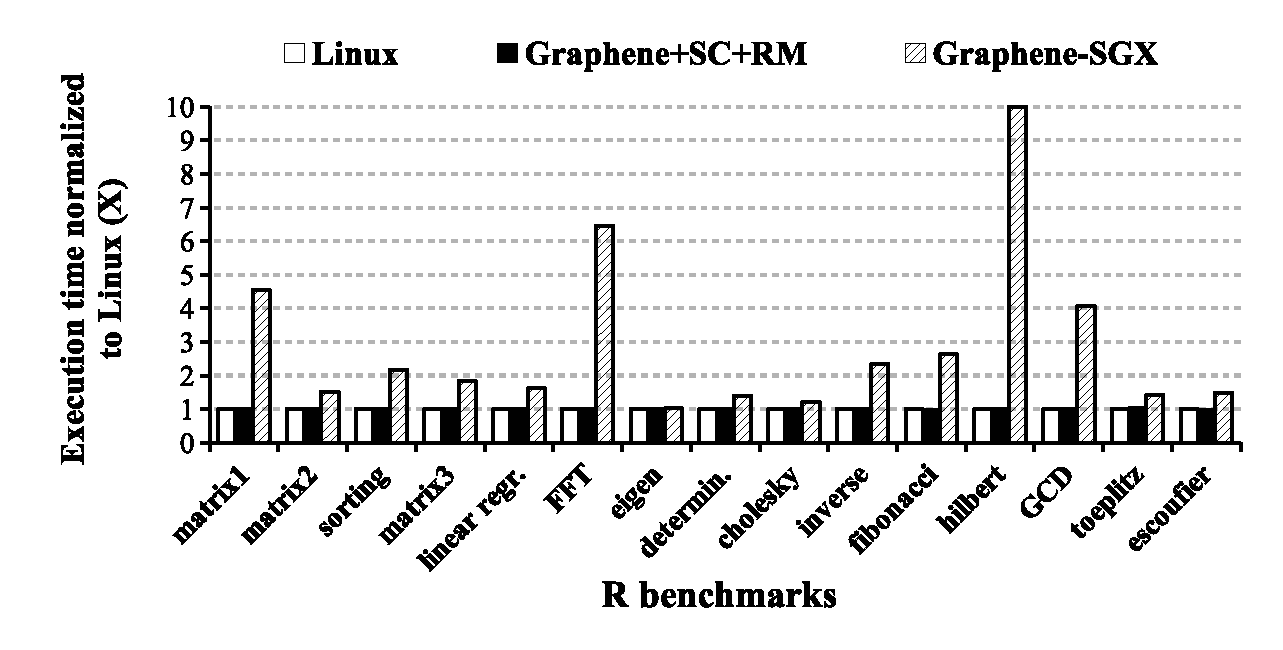
\includegraphics[width=\linewidth]{sgx/r-overhead}\\
{\bf (a) R}
\end{minipage}
\begin{minipage}{.275\textwidth}
\centering
\includegraphics[width=\linewidth]{sgx/gcc-overhead}\\
{\bf (b) GCC}
\end{minipage}
\begin{minipage}{.25\textwidth}
\centering
\includegraphics[width=\linewidth]{sgx/curl-overhead}\\
{\bf (c) CURL}
\end{minipage}

\caption{Performance overhead on desktop applications, including latency of R, execution time of GCC compilation, download time with CURL. The evaluation compares native Linux, \graphene{}, and \graphenesgx{}.} %{\bf Enclave creation time is deducted from the GCC execution time.}}
\label{fig:desktop-overhead}
\end{figure*}



\subsection{Command-Line applications}


We also evaluate the performance of a few commonly-used command-line applications.
%, to evaluate the performance of \graphenesgx{} on PCs instead of servers and clouds.
Three off-the-shelf applications are tested in our experiments:
{\bf R} (v3.2.3) for statistical computing~\cite{r-project}; {\bf GCC} (v5.4), the general GNU C compiler~\cite{gcc}; {\bf CURL} (v7.74), the default command-line web client on UNIX~\cite{curl}.
These applications are chosen because they are frequently used by Linux users,
and each of them potentially  be used 
in an enclave to handle sensitive data---either on a server or a client
machine.
% can realize profitable scenarios of using enclaves on desktop machines.



We evaluate the latency or execution time of these applications. 
%, because desktop users tend to care more about responsiveness than throughput.
In our experiments, both R and CURL have internal timing features to measure the wall time
of individual operations or executions.
%However, for other applications like GCC which does not include internal timing, evaluating the execution time can be influenced by many factors.
On a Linux host, the time to start a library OS is higher than a simple 
process, but significantly lower than booting a guest OS in a VM or
starting a container. 
Prior work measured Graphene (non-SGX) start time at 641 $\mu$s~\cite{tsai14graphene}, whereas starting an empty Linux VM takes 10.3s and starting a Linux (LXC) container takes 200 ms~\cite{agarwal15container}. 
%% dp; Note that this is MILLI seconds, not micro seconds.
%average memory footprint of an empty Linux VM, with memory deduplication, is about 96MB, . 


On SGX, the enclave creation time is relatively higher, \fixme{added more detailed number} ranging from 0.5s (a 256MB enclave) to 5s (a 2G enclave), which is a fixed cost that any application framework
will have to pay to run on SGX.
%For library OSes, the time for creating and initializing an enclave is not trivial, because it is similar to booting an lightweight OS.
% a significant part of the start-up time
% of an application is more significant, because creating enclaves is expensive.
%We consider the enclave creation time as a fixed cost for any application running in \graphenesgx{},
%and acceptable to users as long as it is responsive.
Enclave creation time is determined by the latency of the hardware and the Intel kernel driver, and is primarily a function of the size of 
the enclave, which is specified at creation time because it affects the enclave signature. %\fixmedp{although can't it grow with eadd?}.  
For non-server workloads that create multiple processes during execution,
such as GCC in Figure~\ref{fig:desktop-overhead},
the enclave creation contributes a significant portion to the execution time overheads, illustrated as a stacked bar.
%Since the enclave creation time is related to the enclave size, and unrelated to the workload,
%we deduct the enclave creation time from the execution time of GCC in Figure~\ref{fig:desktop-overhead}. \fixmedp{I think it might be better to show this as a stacked bar instead of just removing it.  Opaquely subtracting this cost doesn't seem right.  Let's discuss dp: I thought we agreed to change this...}

{\bf R}~\cite{r-project} is a scripting language often used for
data processing and statistical computation.
With enclaves, users can process sensitive data on an
OS they don't trust.
We use an R benchmark suite developed by Urbanek et al.~\cite{r-benchmark-25}, which includes 15 CPU-bound workloads such as matrix computation and number processing.
\graphenesgx{} slows down by less than 100\% on the majority of the workloads, excepts the ones which involve allocation and garbage collection: ({\tt matrix1} creates and destroys matrices, and both {\tt FFT} and {\tt hilbert} involve heavy garbage collection.)
Aside from garbage collection, these R benchmarks do not frequently interact with the host.
We further note that non-SGX \graphene{} is as efficient as Linux on all workloads, 
and these overheads appear to be SGX-specific.
%\fixmedp{Check this pontification}
In our experience, garbage collection and memory management code in managed language runtime
systems tends to be written with assumptions that do not match enclaves,
such as a large, sparse address space or that memory can be demand paged 
nearly for free (SGX version 1 requires all memory to be mapped
at creation); a useful area for future work would be to design
garbage collection strategies that are optimized for enclaves.
%we believe the overheads on \graphenesgx{} are contributed by enclaves.
 
{\bf GCC}~\cite{gcc} is a widely-used C compiler.
By supporting GCC in enclaves, developers can compile closed-source applications on customers' machines,
without leaking the source code.
GCC composes of multiple binaries, including {\tt cc1} (compiler), {\tt as} (assembler), and {\tt ld} (linker).
Therefore, GCC is a multi-process program using \syscall{execve}.
We test the compilation of thee source files with varied sizes,
using single C source files collected by MIT~\cite{gcc-benchmark}.
Each GCC execution typically \fixme{it's five, not four} creates five processes, and we run each process in a 256MB enclave by default.
%and has a fixed cost on enclave creation, which is unrelated to workload and depends on the enclave size.
%\fixme{check this}
\fixme{clarified this part, to prevent confusion between latency and overhead. also, GCC numbers got better.}
For a small workload like compiling {\tt gzip.c} (5 kLoC), running in \graphenesgx{} (4.1s) is 18.7$\times$ slower than Linux (0.2s).
The bulk of this time is spent in enclave creation, taking 3.0s in total, while the whole execution inside the enclaves, including initialization of the library OS and OS shield, takes only 1.1s, or 4.2$\times$ overhead.
For larger workloads like {\tt oggenc.c} (50 kLoC) and {\tt gcc.c} (500 kLoC), 
the overhead of \graphenesgx{} is less significant. % (3.6$\times$ and 2.1$\times$ overhead, respectively).
For {\tt gcc.c} (500 kLoC), we have to enlarge one of the enclaves ({\tt cc1}) to 2GB,
but running on \graphenesgx{} (53.1s) is only 2.1$\times$ slower than Linux (17.2s),
and 7.1s is spent on enclave creation.
%and the creation of four enclaves takes 8s.
%Each compilation has a fixed enclave creation time in \graphenesgx{}, which is about 1--2 seconds per enclave. We deduct the creation time of all enclaves  to gain more meaningful results, but do not hide rest of the overhead on fork.
%\fixmedp{Also not comfortable with this; add a bar?}
%In general, GCC in \graphenesgx{} is 1--5$\times$ slower than GCC on native Linux. 
%\fixmedp{This really needs some profiling if possible}
The overhead of non-SGX \graphene{} on GCC is marginal.
 



{\bf CURL}~\cite{curl} is a command-line  web downloader.
\graphenesgx{} can make CURL into a secure downloader that attests both server and client ends.
We evaluate the total time to download a large file, ranging from 1MB to 1GB, from another machine running Apache. % over Gigabit LAN.
%across high-speed university network\fixmedp{more specific, as above}.
\graphene{} has marginal overhead on CURL, and
\graphenesgx{} adds 7--61\% overhead to the downloading time of CURL, due to the latency of I/O.


\begin{figure*}[t!]
\centering

\begin{minipage}{.3\textwidth}
\centering
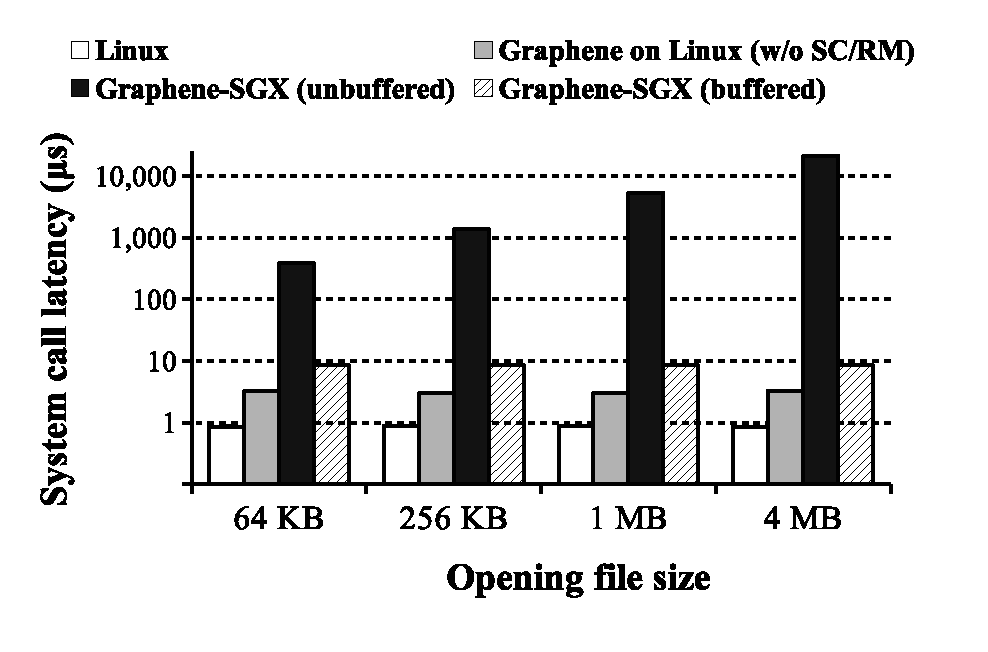
\includegraphics[width=\linewidth]{sgx/open-latency}\\
{\bf (a) Open a file}
\end{minipage}
\begin{minipage}{.3\textwidth}
\centering
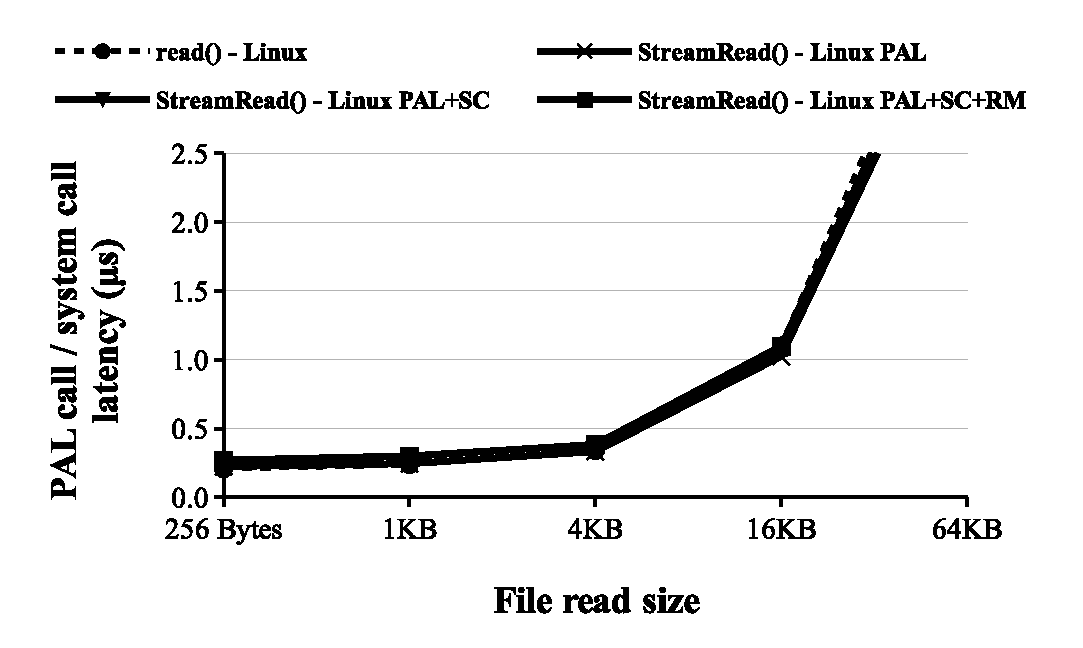
\includegraphics[width=\linewidth]{sgx/read-latency}\\
{\bf (b) Read a file}
\end{minipage}
\begin{minipage}{.3\textwidth}
\centering
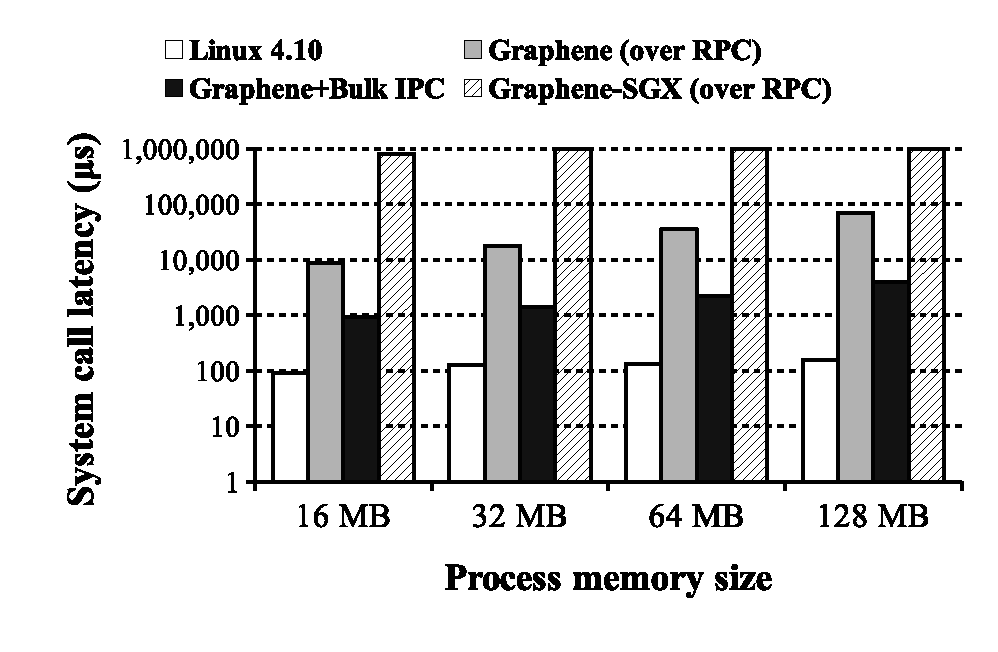
\includegraphics[width=\linewidth]{sgx/fork-latency}\\
{\bf (c) Fork a process}
\end{minipage}

\caption{Latency of some expensive system calls in \graphenesgx{}, including opening and reading a secured (authenticated) file, and forking a new process. The results are compared with native Linux and \graphene{}.}
\label{fig:syscall}
\end{figure*}


\subsection{Performance Overhead Analysis}


In this section we evaluate a few system operations that are heavily impacted by the \graphenesgx{} design.
%To shield dynamic loading and process creation,
%\graphenesgx{} uses computationally-expensive cryptographic techniques \fixmedp{more specific?} to verify enclave inputs.
% under the circumstance that the host OS cannot be trusted.
%As a trade-off to the security, the performance will be affected
%by additional cryptographic computation.
We measure the \syscall{open}, \syscall{read}, and \syscall{fork} system calls
using LMbench 2.5~\cite{McVoy:lmbench}.
A primary source of the overheads on these system calls is the cost of shielding applications, with run-time checks on the inputs.
Cryptographic techniques are used to: (1) validate the file against the secure hash, at \syscall{open}, (2) check the file chunks against the Merkle tree, at \syscall{read}, and (3) establish a TLS connection over inter-enclave RPC, at \syscall{fork}.
%opening a integrity-sensitive file for the first time, 
% or using cryptographic techniques, such as secure hashing, to verify the inputs.
% microbenchmarking specific system calls: 
% system calls,
%with different application settings.
%The microbenchmark is part of the LMBench 2.5 test suite
%\fixmedp{maybe merge this in the above paragraph, which feels a little coy}
%For instance, in order to shield dynamic loading, \graphenesgx{} checks each binary file against the secure hashes in the manifest,
%when the file is opened for the first time---after the whole file is copied into the enclave.
%\fixmedp{This happens after they are copied into enclave, memory right?}
%The verification happens when opening the file for the first time (often by the 
%After \graphenesgx{} validates the file, we generate a series of hashes of the file in chunks, as a merkle tree.
%to prevent verifying the whole file again when later randomly reading a part of the file.
%\fixmedp{So is this for the case when a file is swapped out?  I'm confused here - some details are missing}
%The latency of opening and reading an authenticated file in \graphenesgx{} is dominated by SHA256 and SHA512 calculation.
The remaining overheads contribute to exiting the enclave for host system calls, and bringing memory into the EPC (enclave page cache) or decrypting 
memory on a last-level cache miss. %and later the cache where the memory is decrypted by the CPU.


Figure~\ref{fig:syscall}(a)
shows the overhead for authenticating files in \syscall{open}.
\fixme{change overhead to latency}
Depending on the file size, the latency of \syscall{open} on \graphenesgx{} is 383$\mu$s (64KB file) to 21ms (4MB file), whereas on Linux, the latency is constant at 0.85$\mu$s.
We note that this is where enclaves are at a disadvantage, as \syscall{open} 
normally does not need to read file content; whereas here \graphenesgx{} uses \syscall{open}
as a point at which to validate file content.
For a subsequent \syscall{open}, when the Merkle tree is already generated, the overhead of simply exiting enclave for \syscall{open}, and searching the file list in the manifest, is about 9$\times$.
%\fixmedp{why?}


One might be able to optimize further for cases where only part of a file is accessed
with incremental hashing.  However, in the common case where nearly all of the file is accessed,
these costs are difficult to avoid when host file system is untrusted.
Another opportunity 
is to create the Merkle tree offline, when the manifest is created.
%\fixmedp{I think the second idea has legs...}


%This is an inevitable cost, because normal \funcname{open} on trusted OSes
%need not to access file content.
%After verifying the file, \graphenesgx{} buffers the chunk hash values, to skip whole-file verification when the file is reopened.

Figure~\ref{fig:syscall}(b)
shows the overhead for authenticating files in \syscall{read}, which 
is lower than \syscall{open}.
Since the whole file has been verified at \syscall{open}, the sequential \syscall{read} only verifies the chunks of files it is reading from untrusted memory.
%Reads from data cached in enclave memory are cheaper.  %\fixmedp{right? can we say how much cheaper?  Maybe add separate bars for both cases?}
% Therefore, \syscall{read} is actually much cheaper than \syscall{open}.
Depending on the size of blocks being read, the latency on \graphenesgx{} is 0.5$\mu$s (64-byte \syscall{read}) to 16.9$\mu$s (4KB \syscall{read}). The latency of \syscall{read} on Linux is \roughly{}0.1$\mu$s for any block size below 4KB.
If the file is not authenticated,
\graphenesgx{} only copies the file contents into the buffer, and the overhead reduces to 48\% (64-byte \syscall{read}) to 83\% (4KB \syscall{read}).
\fixmedp{Consider doing larger buffers, say up to 64k or even 4 MB}

%\fixmedp{In the legend for 7b, unsecure should be insecure}


Figure~\ref{fig:syscall}(c) shows the overhead of forking a process.
As described in \ref{sec:multiproc}, the latency of \syscall{fork} in \graphenesgx{} is affected by three factors:
creation of a new enclave, local attestation of the integrity, and duplicating the process state over an encrypted RPC stream.
Combining these factors, \syscall{fork} is one of the most expensive calls in \graphenesgx{}.
%, but at least it is supported natively on the current hardware.
The default enclave size is 256MB.
%which takes \roughly{}0.5s to create. 
Our evaluation shows that the latency of forking a process is around 0.8s (16MB process) to 2.7s (128MB process), but can be more expensive if the parent process uses more memory.
The trend matches the performance of \graphene{} without the bulk IPC optimization.
\fixmedp{If you want, some thoughts on how this might be improved in the future would be nice...  One good suggestion is recycling enclaves, or pre-forking so measurements can be done in parallel}
%Due to the overhead on \funcname{fork}, \graphenesgx{} is not suitable for fork-intensive workloads like Bash scripts
%if performance is critical.

\fixme{talk about a limitation of improving fork. check this.}
One way to further optimize \syscall{fork} is to reduce or avoid enclave creation time; one can potentially pre-launch a child enclave, and then migrate the process contents later when \syscall{fork} is called.
There might be another opportunity to improve the latency of process migration,
if copy-on-write sharing of enclave pages can be supported in future generations of SGX.
%Unfortunately, sending the process contents is difficult to avoid in \syscall{fork},
%as SGX disallows sharing enclave memory between multiple enclaves.

%\fixmedp{I assume 5.4 isn't done yet}



\subsection{TCB Size and Shielded Functionality}

In this section we measure the increase in TCB size of \graphenesgx{},
%in lines of code, 
as well as 
%compare the TCB size increased by \graphenesgx{} to an unmodified application, in lines of code, and 
the OS functionality shielded by the framework.
We compare to \scone{} and \panoply{}, using
%For SCONE and Panoply, we use 
numbers reported in their papers. 
%The conventional One generally assumes 
A smaller TCB is generally easier to review or possibly verify,
and is assumed to have fewer vulnerabilities.
%more implies lower burden for code review or formal verification, and less risk of writing exploitable code.
%For instance, Panoply argues that, because its use cases are typically smaller than 20kLoC, including both the application logic and Panoply itself, it is within the realm of future, automated verification~\cite{shinde17panoply}.

\fixmedp{Reviewer B asks for memory footprint, which isn't a bad idea}

\begin{table}
\footnotesize
\centering
\bgroup
\def\arraystretch{1.2}
\setlength{\tabcolsep}{0.5em}
\begin{tabular}{>{\raggedright\arraybackslash}p{9em}>{\raggedleft\arraybackslash\bf}p{7em}>{\raggedleft\arraybackslash}p{4.25em}>{\raggedleft\arraybackslash}p{4.25em}}
Components                    & \graphenesgx{}  & \scone{}     & \panoply{}  \\
\hline
libc (ld, libm, pthread)      &  1,292 &   88 & --      \\
                              & (glibc-2.19) & (musl)   &          \\
Library OS                    &     34 &  --      & --     \\
PAL / OS Shield               &     22 &   99 & 10  \\
\hline
Total                         &  1,348 &  187 & 10  \\
\hline
\end{tabular}
\egroup
\caption{TCB size (in thousands of lines of code) of \graphenesgx{}, \scone{}, and \panoply{}.}
\label{tab:tcb-size}
\end{table}

Table~\ref{tab:tcb-size} lists the lines of code in each components within the TCB of \graphenesgx{}, \scone{}, and \panoply{}.
By comparing the total TCB size, \graphenesgx{} is 9$\times{}$ larger than \scone{}, and 134$\times{}$ larger than \panoply{}.
However, the primary difference is the selection of libc: 
for maximum compatibility, \graphene{} uses glibc.
\scone{} uses the smaller musl libc, which lacks some features of glibc.
%it would be easy to use the smaller, and incomplete, musl libc.
%SCONE uses 
% Linux applications, \graphenesgx{} chooses to use a minimally-modified glibc, whereas SCONE uses the much more lightweight musl and 
\panoply{} excludes libc from its TCB,
% \fixmedp{what is their rationale, again? Check this}
to fit into the range of automated formal verification,
as they shield at the libc interface.
In principle, \graphene{} could easily support musl as well as glibc for applications
that do not need the additional features of glibc.
We also see the benefit of removing unused code from 
libraries, especially in an unsafe language,
similar to the approach taken in unikernels~\cite{unikernels}.
On balance, 
this choice of libc implementation is largely orthogonal to the issue
of how general-purpose the shields are.

%We argue that the choice of libc is orthogonal to the design of \graphenesgx{}; one can statically compile the applications against musl or glibc if TCB size is a concern, or given plenty of time, trim the libc functionality to bare minimum. 

If we focus on the TCB size of the library OS and the shields, 
\graphenesgx{} is 
%library OS and PAL in \graphenesgx{}, with the shielding layer of SCONE, we are 
44\% smaller than \scone{}. 
We cannot analyze the size of \scone{} because it is closed source.
%, although
%we suspect
%Although it is unclear what is in the implementation of SCONE, because it is not yet open-sourced, we believe the largest portion of their TCB contributes to the cryptography library.
\panoply{} has a smaller TCB in its shield, but within the same order of magnitude.
Panoply only shields 91 out of 256 supported POSIX functions; for context, POSIX 1003.1 defines 1,191 APIs~\cite{POSIX1003-1-2008}.
%out of 256 currently supported by \panoply{} \fixmedp{The better number is how many total functions in POSIX}.

All three of these compatibility layers or shields are within the same
order of magnitude in code size, and the differences are likely 
correlated with different ranges of supported functionality.
A recent study indicates that only order-of-magnitude differences in code
size correlate with reported CVE vulnerabilities; within the same order-of-magnitude,
the data is inconclusive that there is a meaningful difference in risk~\cite{security-metric}.
Thus, increased generality does not necessarily come with 
increased risk. % is not a clear relationship between risk 

% data only correlates
%with differences in code size when 

%Besides the choice of libc, we argue that the TCB size of a library OS or a shim shielding layer is actually correlated with the functionality that it supports or shields. Because none of the three frameworks have completely shielded the whole Linux system call table or POSIX, it is unclear how much code has to be added in the future. \graphenesgx{} also shows that one can always engineer a library OS with a small TCB, if most code is not reused from a monolithic OS kernel like Windows or Linux.
%A recent study of the CVE database also points out that having a larger TCB does not necessarily indicate more vulnerabilities, even when the difference is more than two order-of-magnitude. 



\input{apistudy}

\makeatletter
\def\input@path{{}}
\makeatother
\graphicspath{{}}
\section{Summary}



The Linux PAL successfully leverages a limited subset of Linux system calls,
to implement the whole PAL ABI for running a
full-featured \libos{}.
\Thehostabi{} separates the development of a host OS or hypervisor
from the complexity of emulating a sufficiently-compatible
Linux kernel.
The chapter shows that most calls in \thehostabi{}
can be directly translated to similar system calls on a Linux host kernel.
Only a few \hostapis{}, such as process creation and inter-thread synchronization, require additional attention for developing an efficient implementation strategy.



The Linux PAL also enforces robust security isolation
between mutually-untrusting applications,
by placing applications in separate, VM-like sandboxes.
The security isolation on a Linux host is based on system call restriction using a \seccomp{} filter, and a trusted reference monitor. % for checking resource access.
Security isolation at the host interface
restricts an untrusted application to explore vulnerable execution paths
inside a Linux kernel.
A \seccomp{} filter 
enforce a fixed, minimal system call profile, regardless of bloated dependency of an application.
The reference monitor follows
simple, white-listed manifest rules listing 
all the authorized files and network addresses of an application,
using well-known semantics
such as AppArmor~\cite{apparmor} or iptable-like firewall rules~\cite{iptablesman}.
The reference monitor can further enforce dynamic, process-specific isolation by splitting a sandbox
to run a child \picoproc{} under more restricted
resource permissions.
\graphene{} on a Linux host can serve as a sandbox framework
with a reduced attack surface
upon the host kernel.







